\documentclass[compress]{beamer}
\usepackage[ngerman]{babel}
\usepackage{graphicx}
\usepackage{subfiles}
\usepackage{listings}

\graphicspath{{images/}}

% \setbeameroption{show notes}

\usetheme[noflama]{custom}

\title{Virtualisierte Arbeitsumgebung für den Test verteilter Systeme}
\subtitle{Microservice-Architektur mit Docker, Kafka, Clojure \& Elm}
\author{Jan-Philipp Willem}
\institute{Fakultät für Informatik\\Hochschule Mannheim}
\date{21. Juni 2017}

\begin{document}

% \begin{frame}[noframenumbering,plain]
% \end{frame}

\maketitle

% \begin{frame}[noframenumbering,plain]{Project-Repository}
% \includegraphics[width=0.8\textwidth]{google.pdf}
% \end{frame}

\section*{Gliederung}
\begin{frame}[noframenumbering,plain]{Gliederung}
  \tableofcontents[hideallsubsections]
\end{frame}

\section{Kontext}
\begin{frame}{Bisheriger Ablauf}
  \begin{itemize}
    \item Student soll (verteilte) Aufgaben programmieren
    \item Es wird die Benutzung von schwergewichtigen IDEs vorgeschlagen
    \item Eclipse, Netbeans bieten Integrationen zu diversen Servern/Technologien
    \item Funktionsweise kann in gegebener (Dev-)Umgebung getestet werden
  \end{itemize}
  \begin{itemize}
    \item Gefahr: keine echte Verteilung
    \item Umgebung verschieden zu Production
    \item Ergebnis kann sich erheblich unterscheiden (Seiteneffekte,..)
    \item Einrichtung der Dev-Umgebung kann dennoch schwierig sein
  \end{itemize}
\end{frame}
\begin{frame}{Anforderungen}
  \begin{itemize}
    \item Dozent beschreibt mit generischer Lösung ein Experiment mit fester Anzahl an Instanzen
    \item Pro Instanz: Angabe von Name, Ports, Standard-Command
    \item Studenten sollen mithilfe der Experimente gewisse Aufgaben lösen
    \item Getrennte Netzwerke zwischen Experimenten und nach Außen
    \item Upload von Programmpaketen im Webend
    \item Angabe von Main-Class und Argumentenliste
    \item Einzelnes Starten der Instanzen
    \item Ausgabe der dabei geschehenen Logs (stdout, stderror)
  \end{itemize}
\end{frame}
\begin{frame}{Erhoffte Vorteile}
  \begin{itemize}
    \item Dev-Umgebung zum Starten der Instanzen muss nicht zwingend eingerichtet werden
    \item Konsistentes UI des Tools zwischen Aufgaben \break (\& Vorlesungen?)
    \item Durch Hochladen der Programmpakete pro Instanz wird Verteilung auf Netzwerkebene (hoffentlich) besser wahrgenommen
    \item Hostnamen der Instanzen nicht localhost
  \end{itemize}
\end{frame}

\section{Docker}
\begin{frame}{Description}
  \begin{itemize}
    \item Software zum Deployment von Applikationen innerhalb von Containern
    \item Ähnelt Vorgehensweise von Virtuellen Maschienen
    \item Im Gegegsatz: Mithilfe von Docker-Deamon laufen Prozesse direkt auf Host-OS
    \item Dennoch isoliert (CGroups, Kernel Namespaces, SELinux, AppArmor,..)
    \item Keine spezifische Infrastruktur vorgeschrieben (bspw. ESXi)
    \item Beste Unterstützung durch Linux-Derivat (Kernel-Tricks)
    \item Mittlerweile lauffähige Konzepte auf Osx, Windows
  \end{itemize}
\end{frame}
\begin{frame}{Container}
  \begin{itemize}
    \item Deskriptive \& triviale Beschreibung eines Systems und dessen Bestandteile (Rezept)
    \item Instruktionen um Abhähigkeiten zu installieren, Konfigurationen vorzunehmen und Build-Steps auszuführen
    \item Kein Transferieren von großen Builds nötig, da Image durch Dockerfile erzeugbar
    \item Granulare Sub-Images
    \item Trägt implizit zur Dokumentation bei: Jede Änderung an einem Container muss im Rezept ergänzt werden!
  \end{itemize}
\end{frame}
\begin{frame}{Dockerfile}
  \AddToShipoutPictureFG*{%
    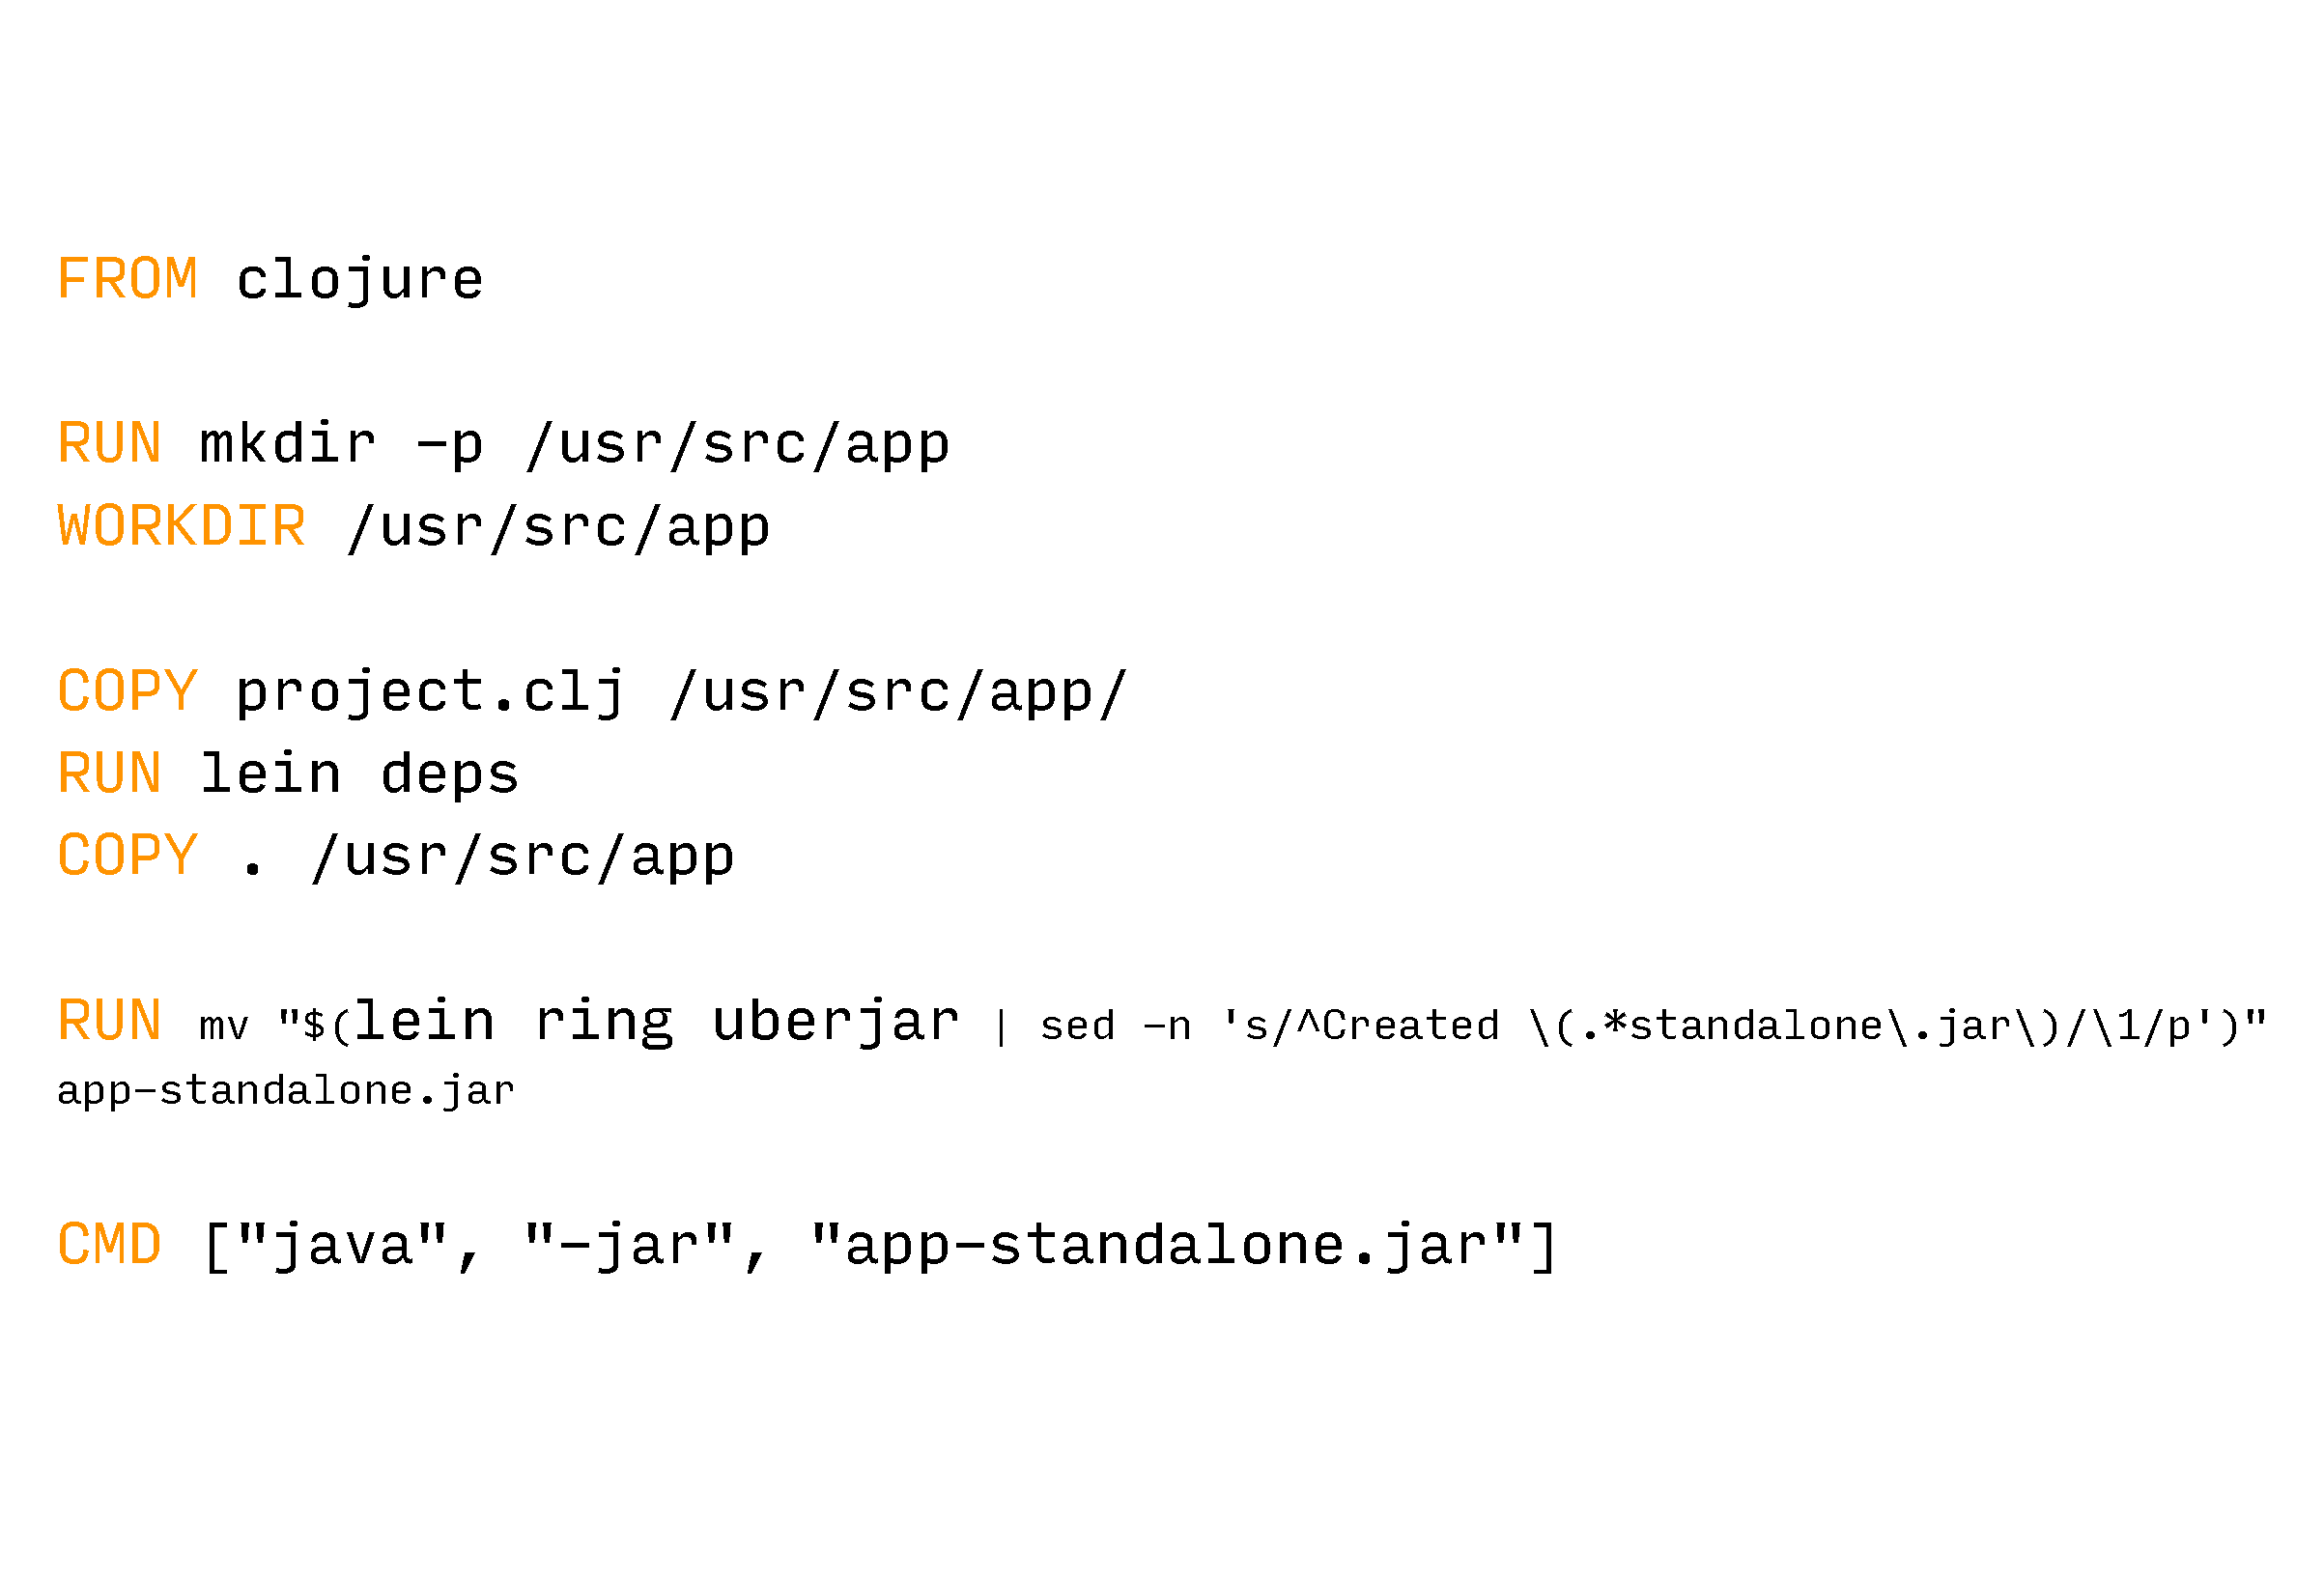
\includegraphics[width=\paperwidth,height=\textheight]{dockerfile.pdf}
  }
\end{frame}
\begin{frame}{Docker-Compose}
  \begin{itemize}
    \item Tool zur Unterstützung von Docker-Cli
    \item Definition von Services als Bestandteil einer App
    \item Ergänzende Angabe von Konfigurations-Parametern an Containern: Volume-Mounts, Ports, Env-Vars, Netzwerke,..
    \item Muss sonst bei \texttt{docker exec} Command angegeben werden
    \item Getrennte Environments für Dev, Test, Prod: \texttt{docker-compose[.dev].yml}
    \item Zentrale Dokumentation!
  \end{itemize}
\end{frame}

\section{Inspiration}
\begin{frame}{Tmux Panes}

  % \AddToShipoutPictureFG*{%
  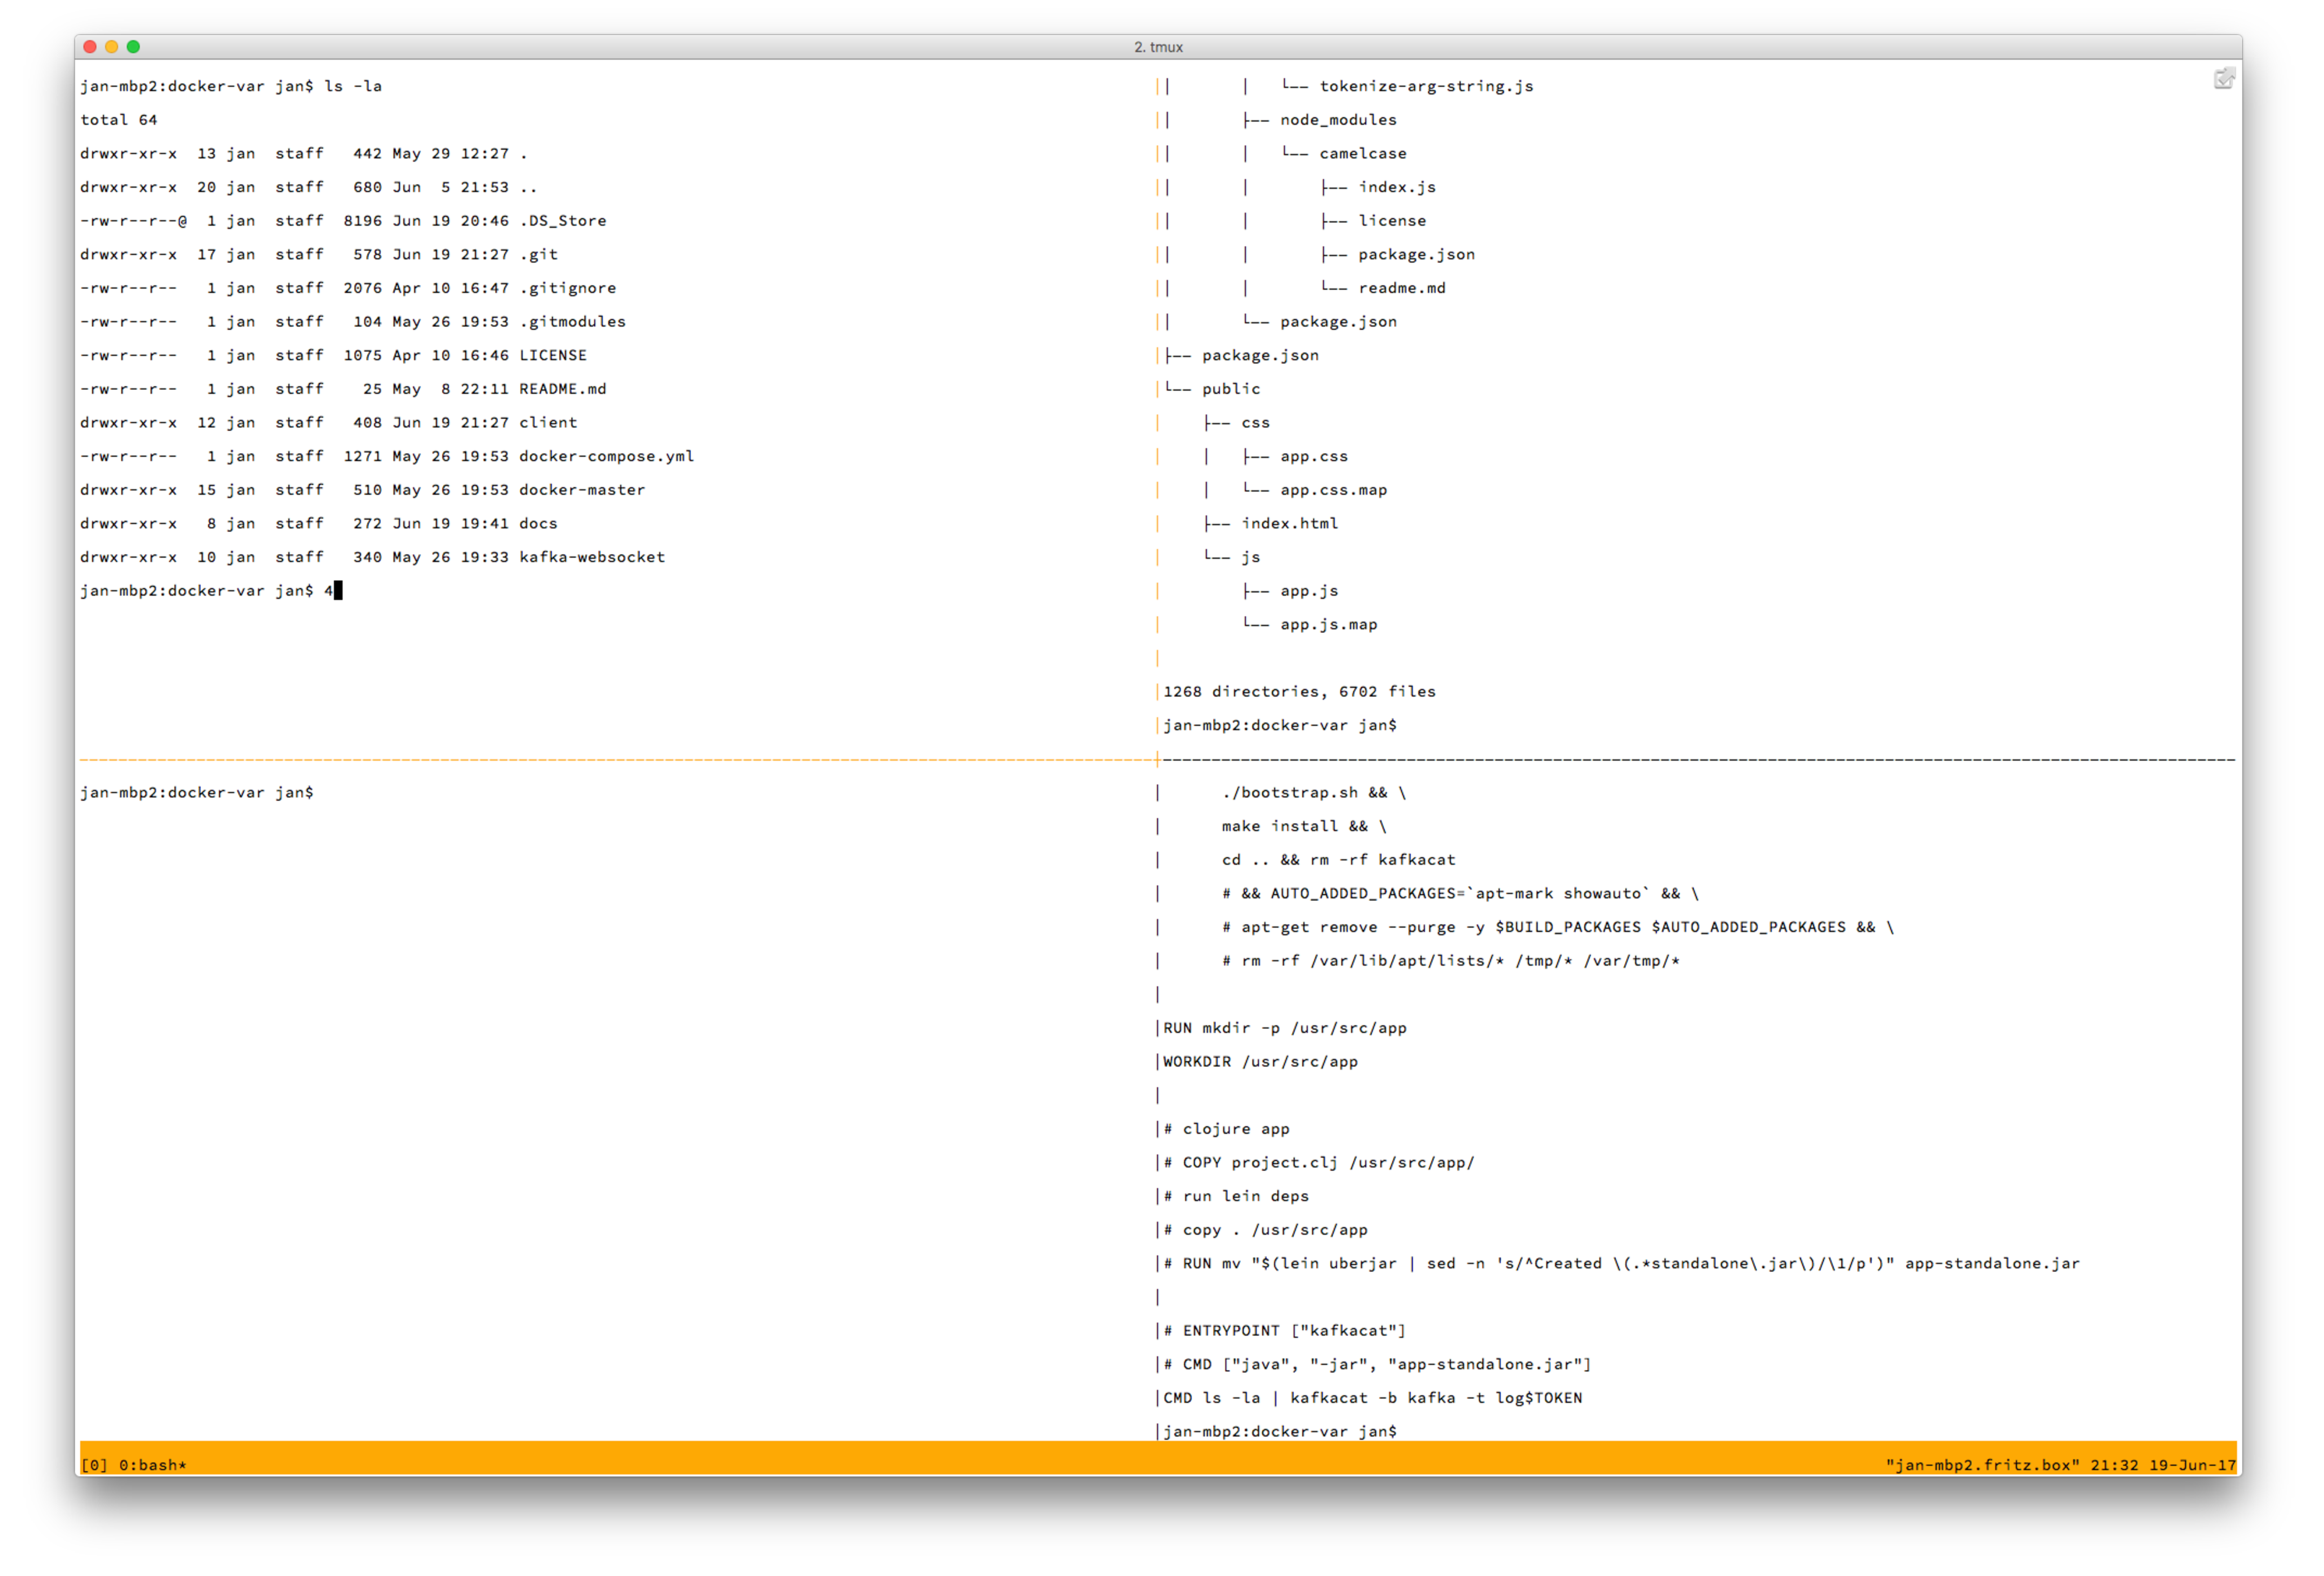
\includegraphics[width=\textwidth]{tmux.pdf}
  % }
\end{frame}
\begin{frame}{Cloud-IDEs}
  \begin{columns}
    \column{.5\textwidth}
    \begin{itemize}
      \item Cloud 9
      \item Source Lair
      \item Eclipse Che
      \item ...
    \end{itemize}

    \column{.5\textwidth}
    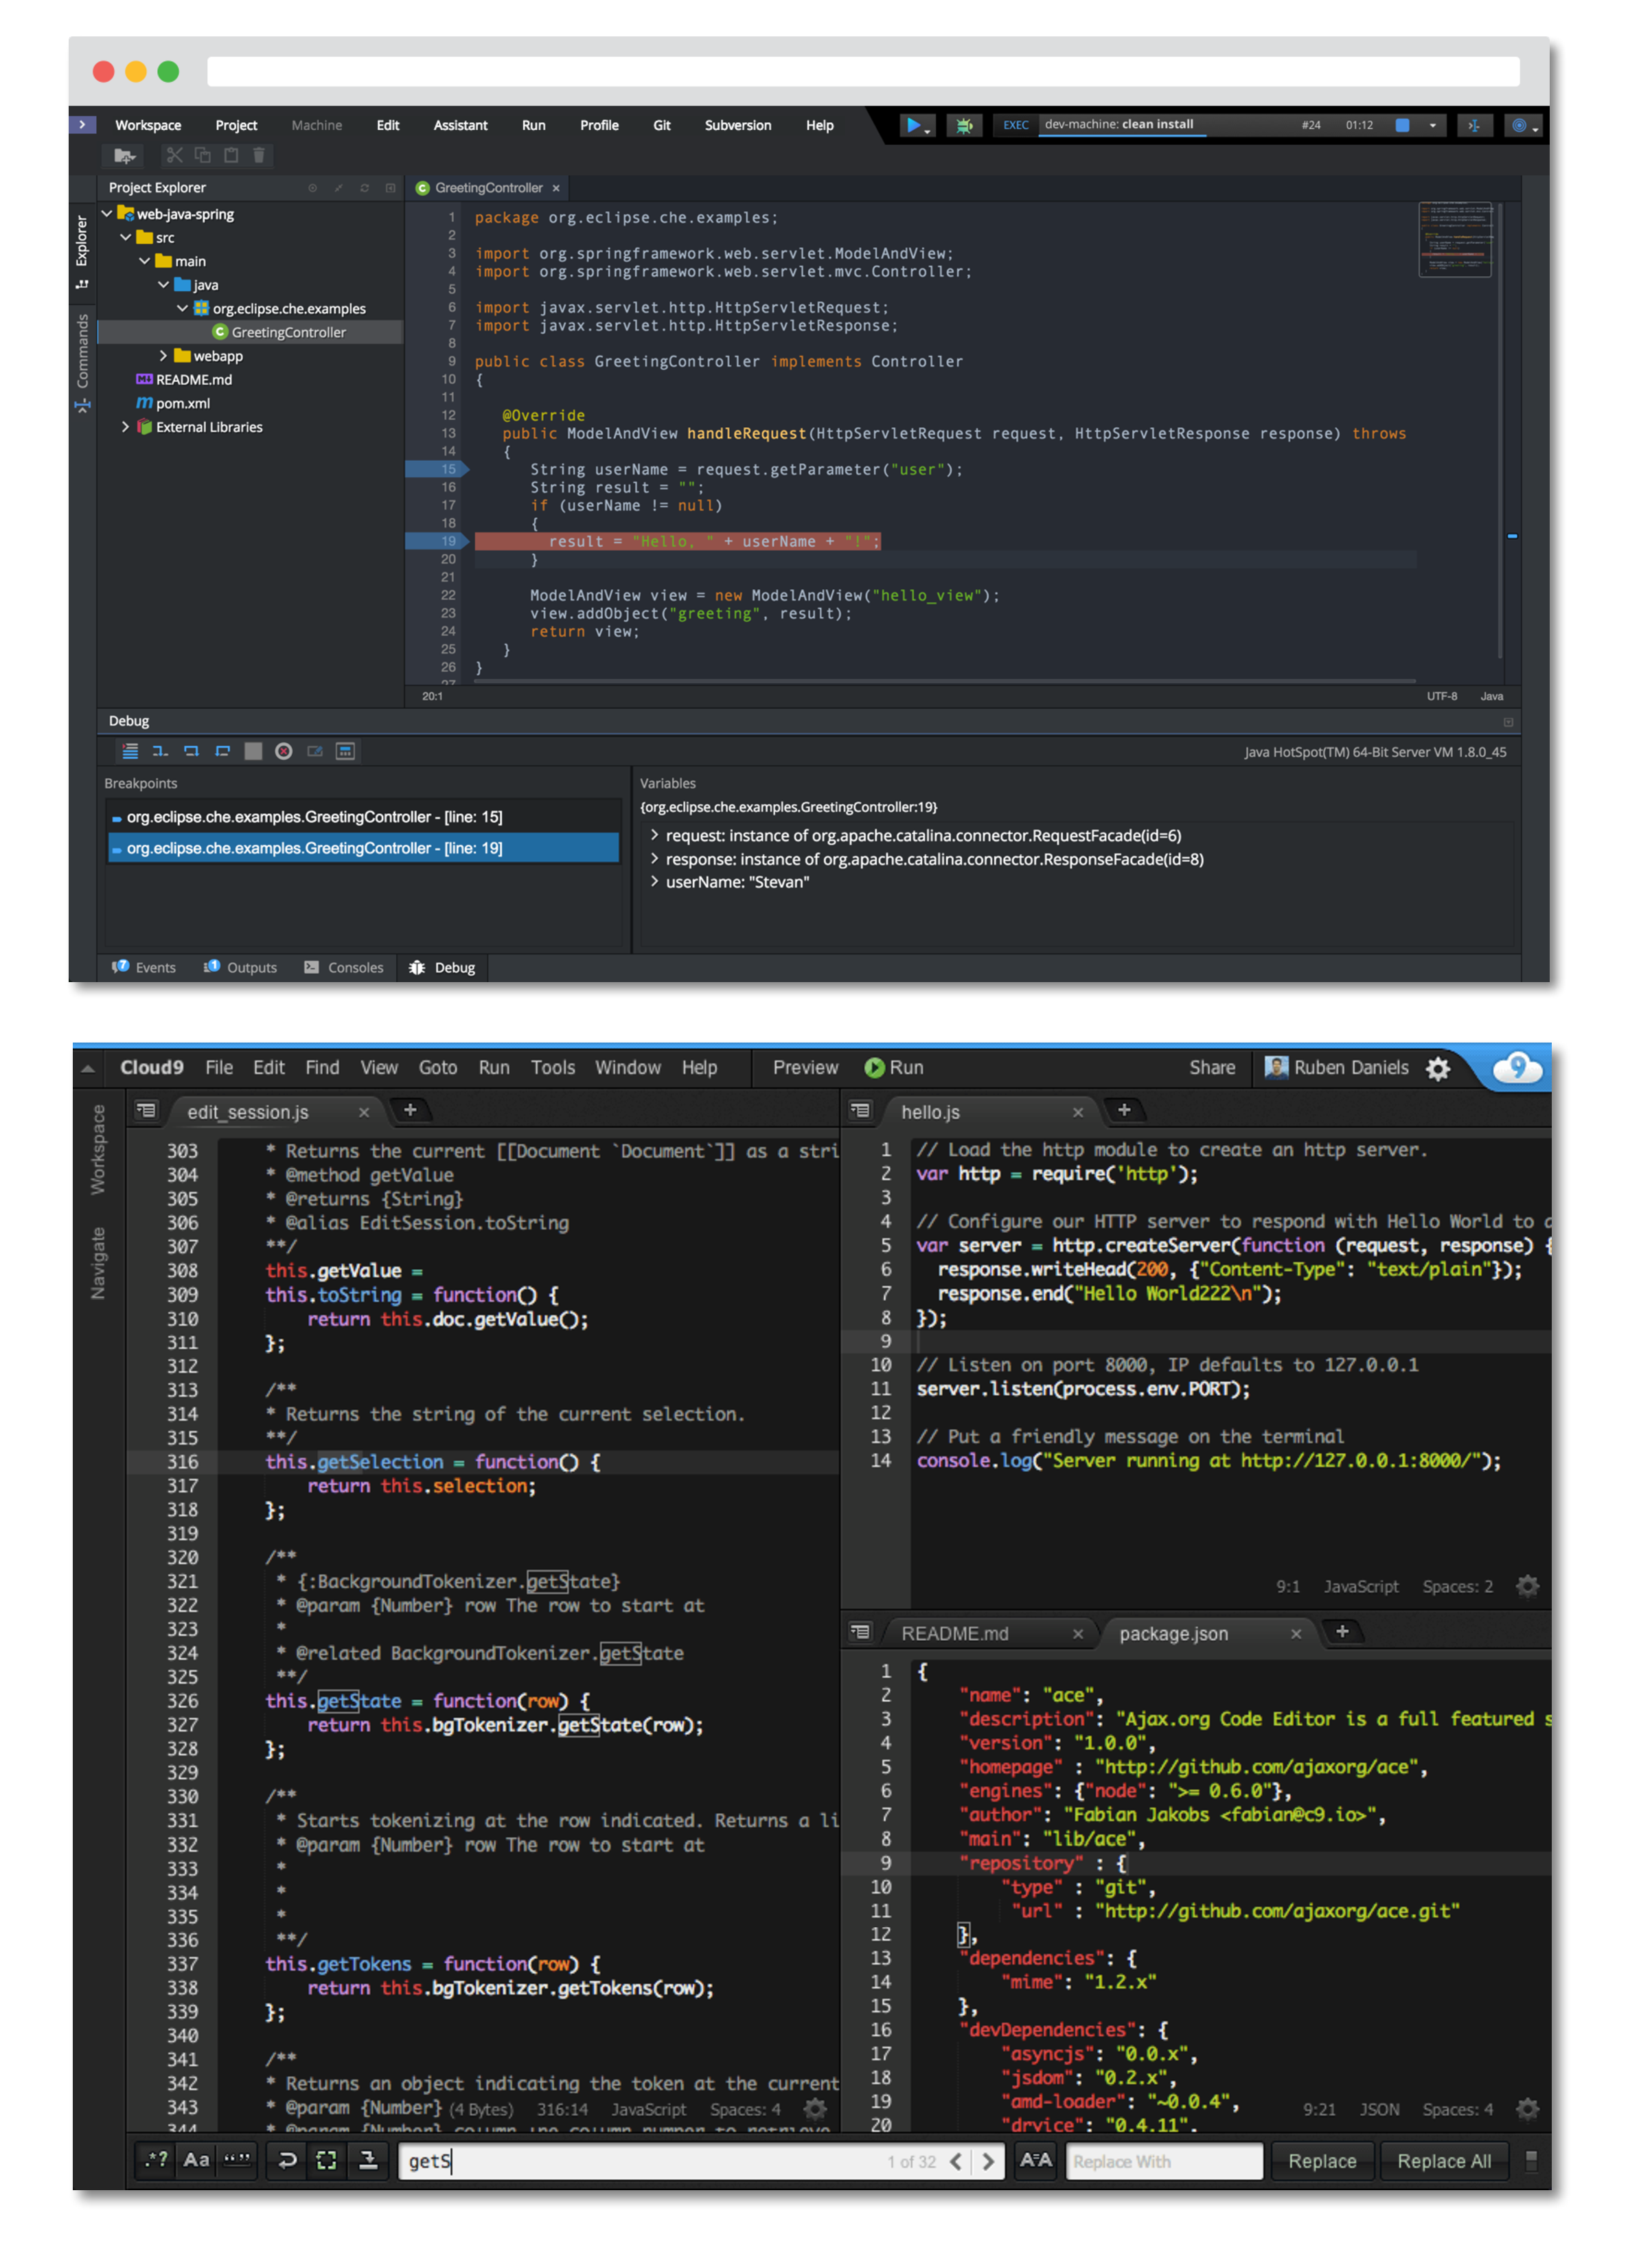
\includegraphics[width=\textwidth]{eclipse.pdf}
  \end{columns}
\end{frame}
\begin{frame}{xterm.js}
  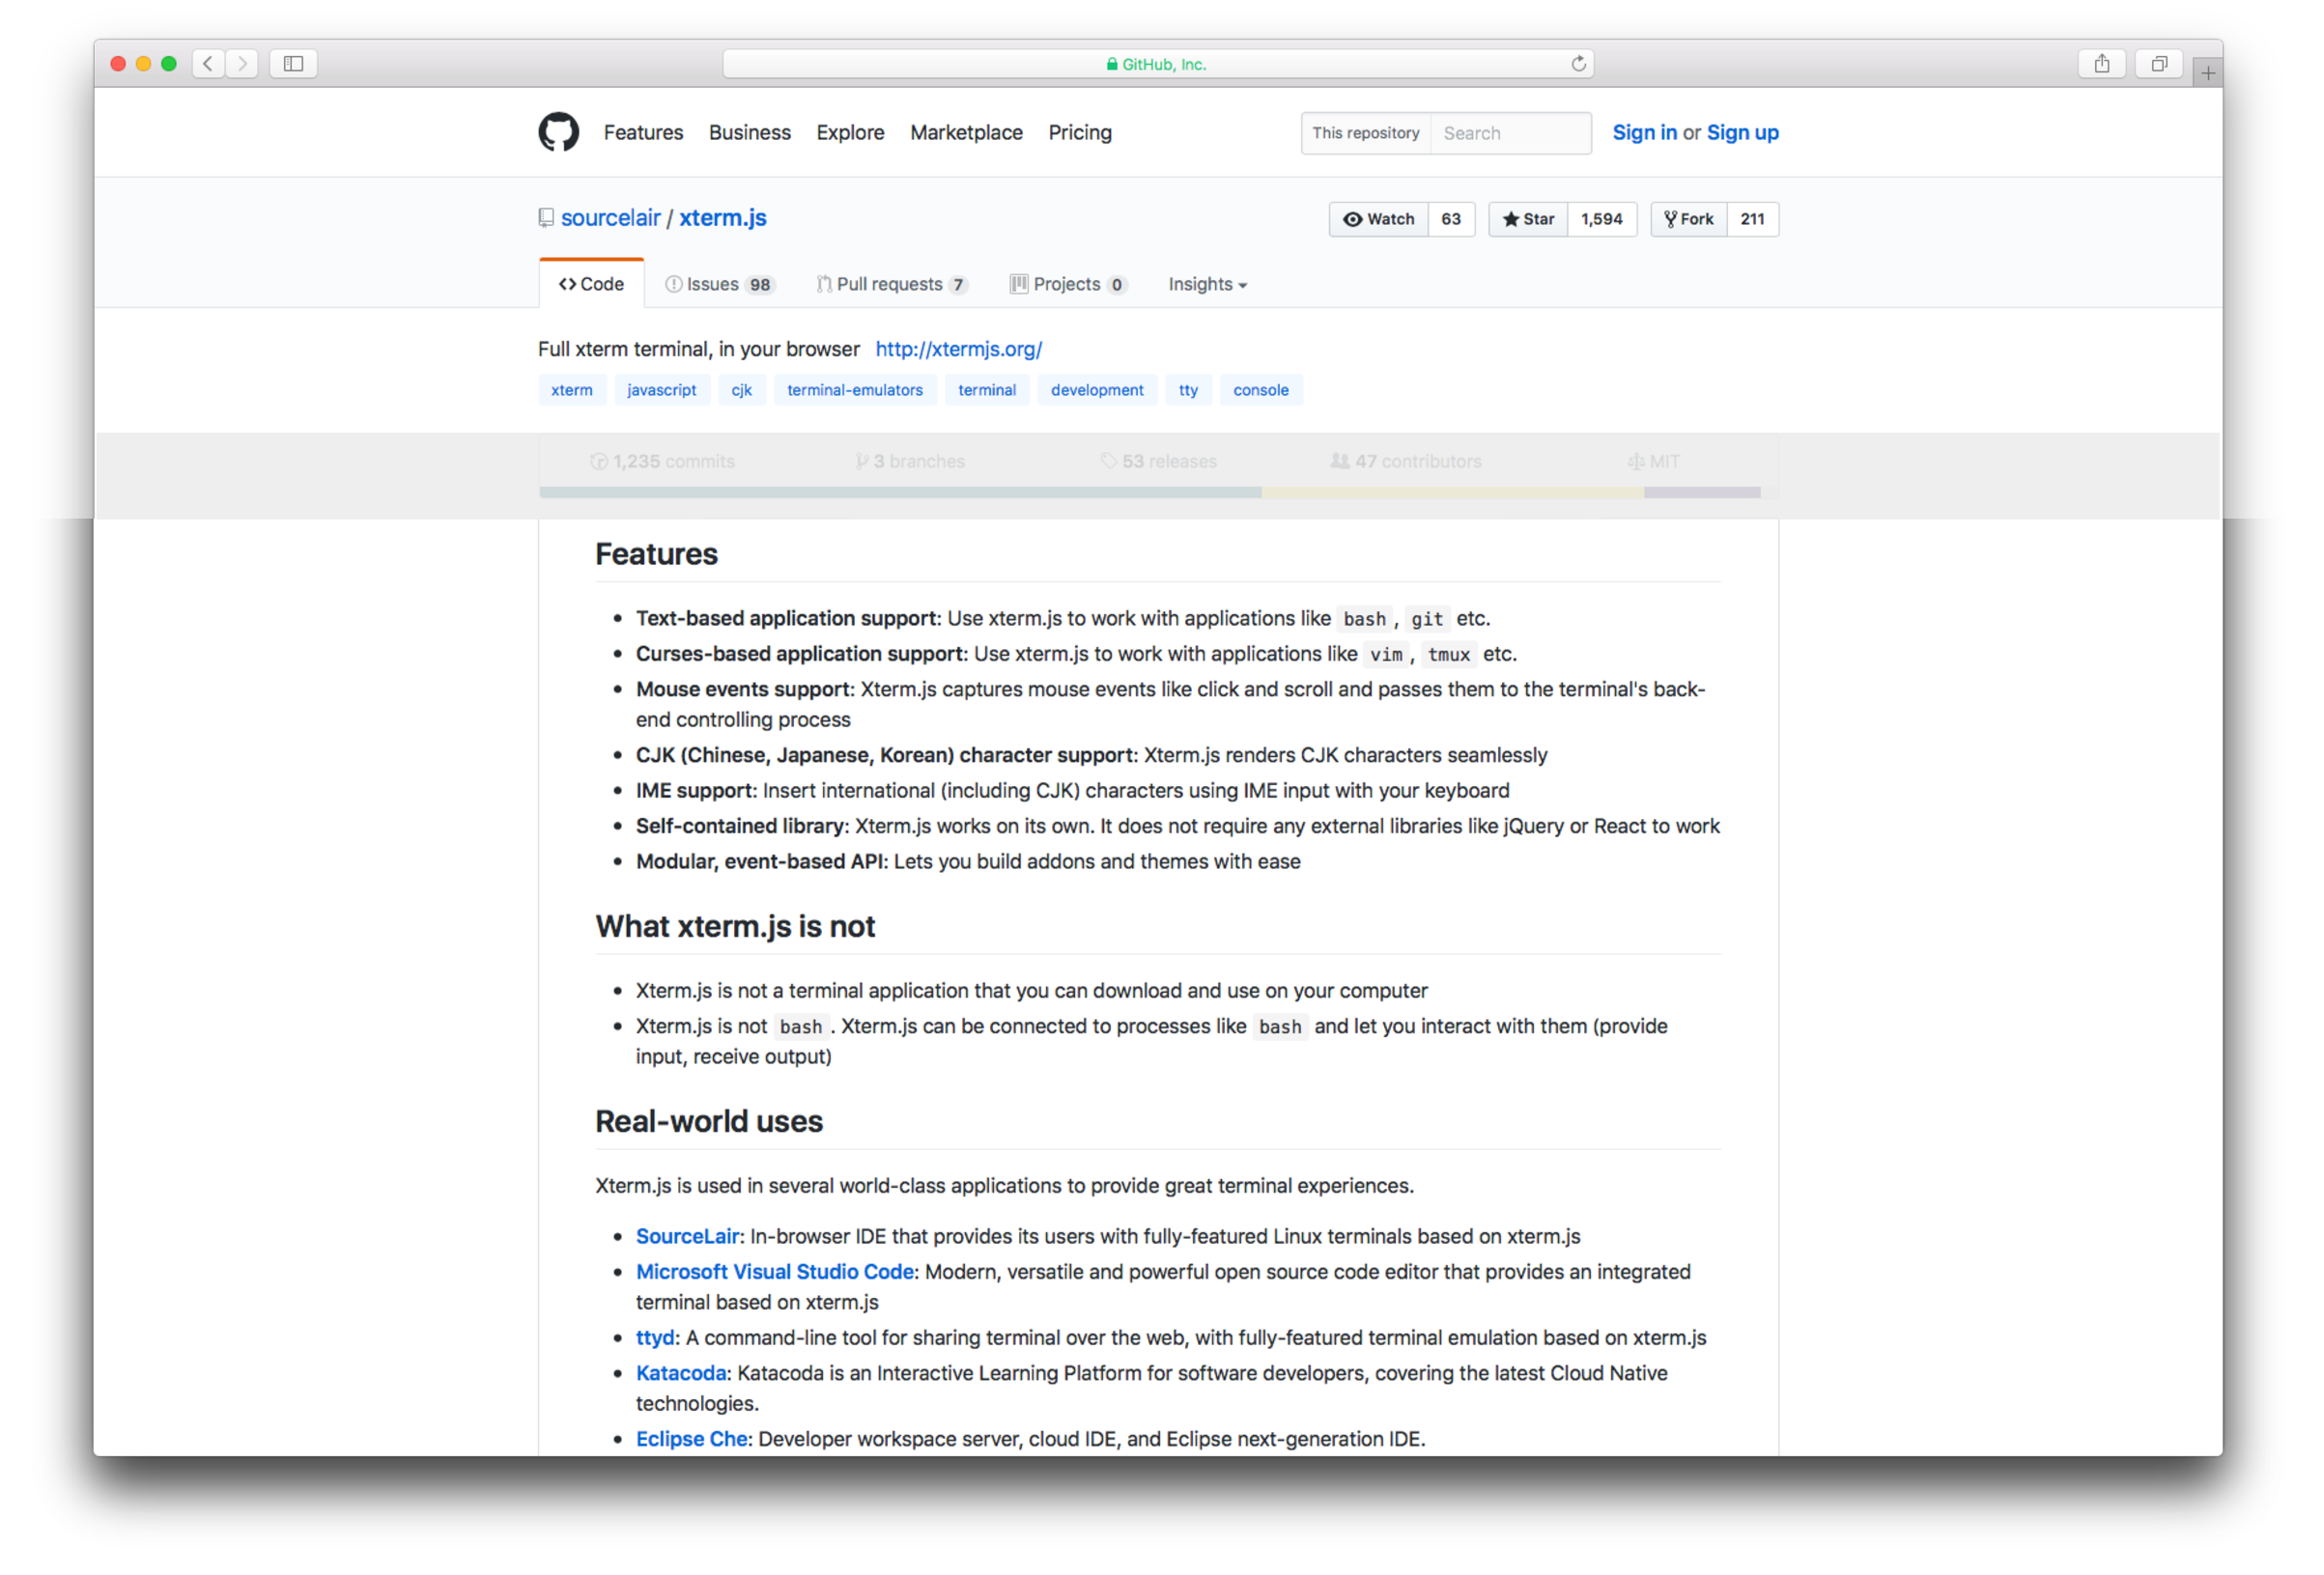
\includegraphics[width=\textwidth]{xterm.pdf}
\end{frame}
\begin{frame}{ttyd}
  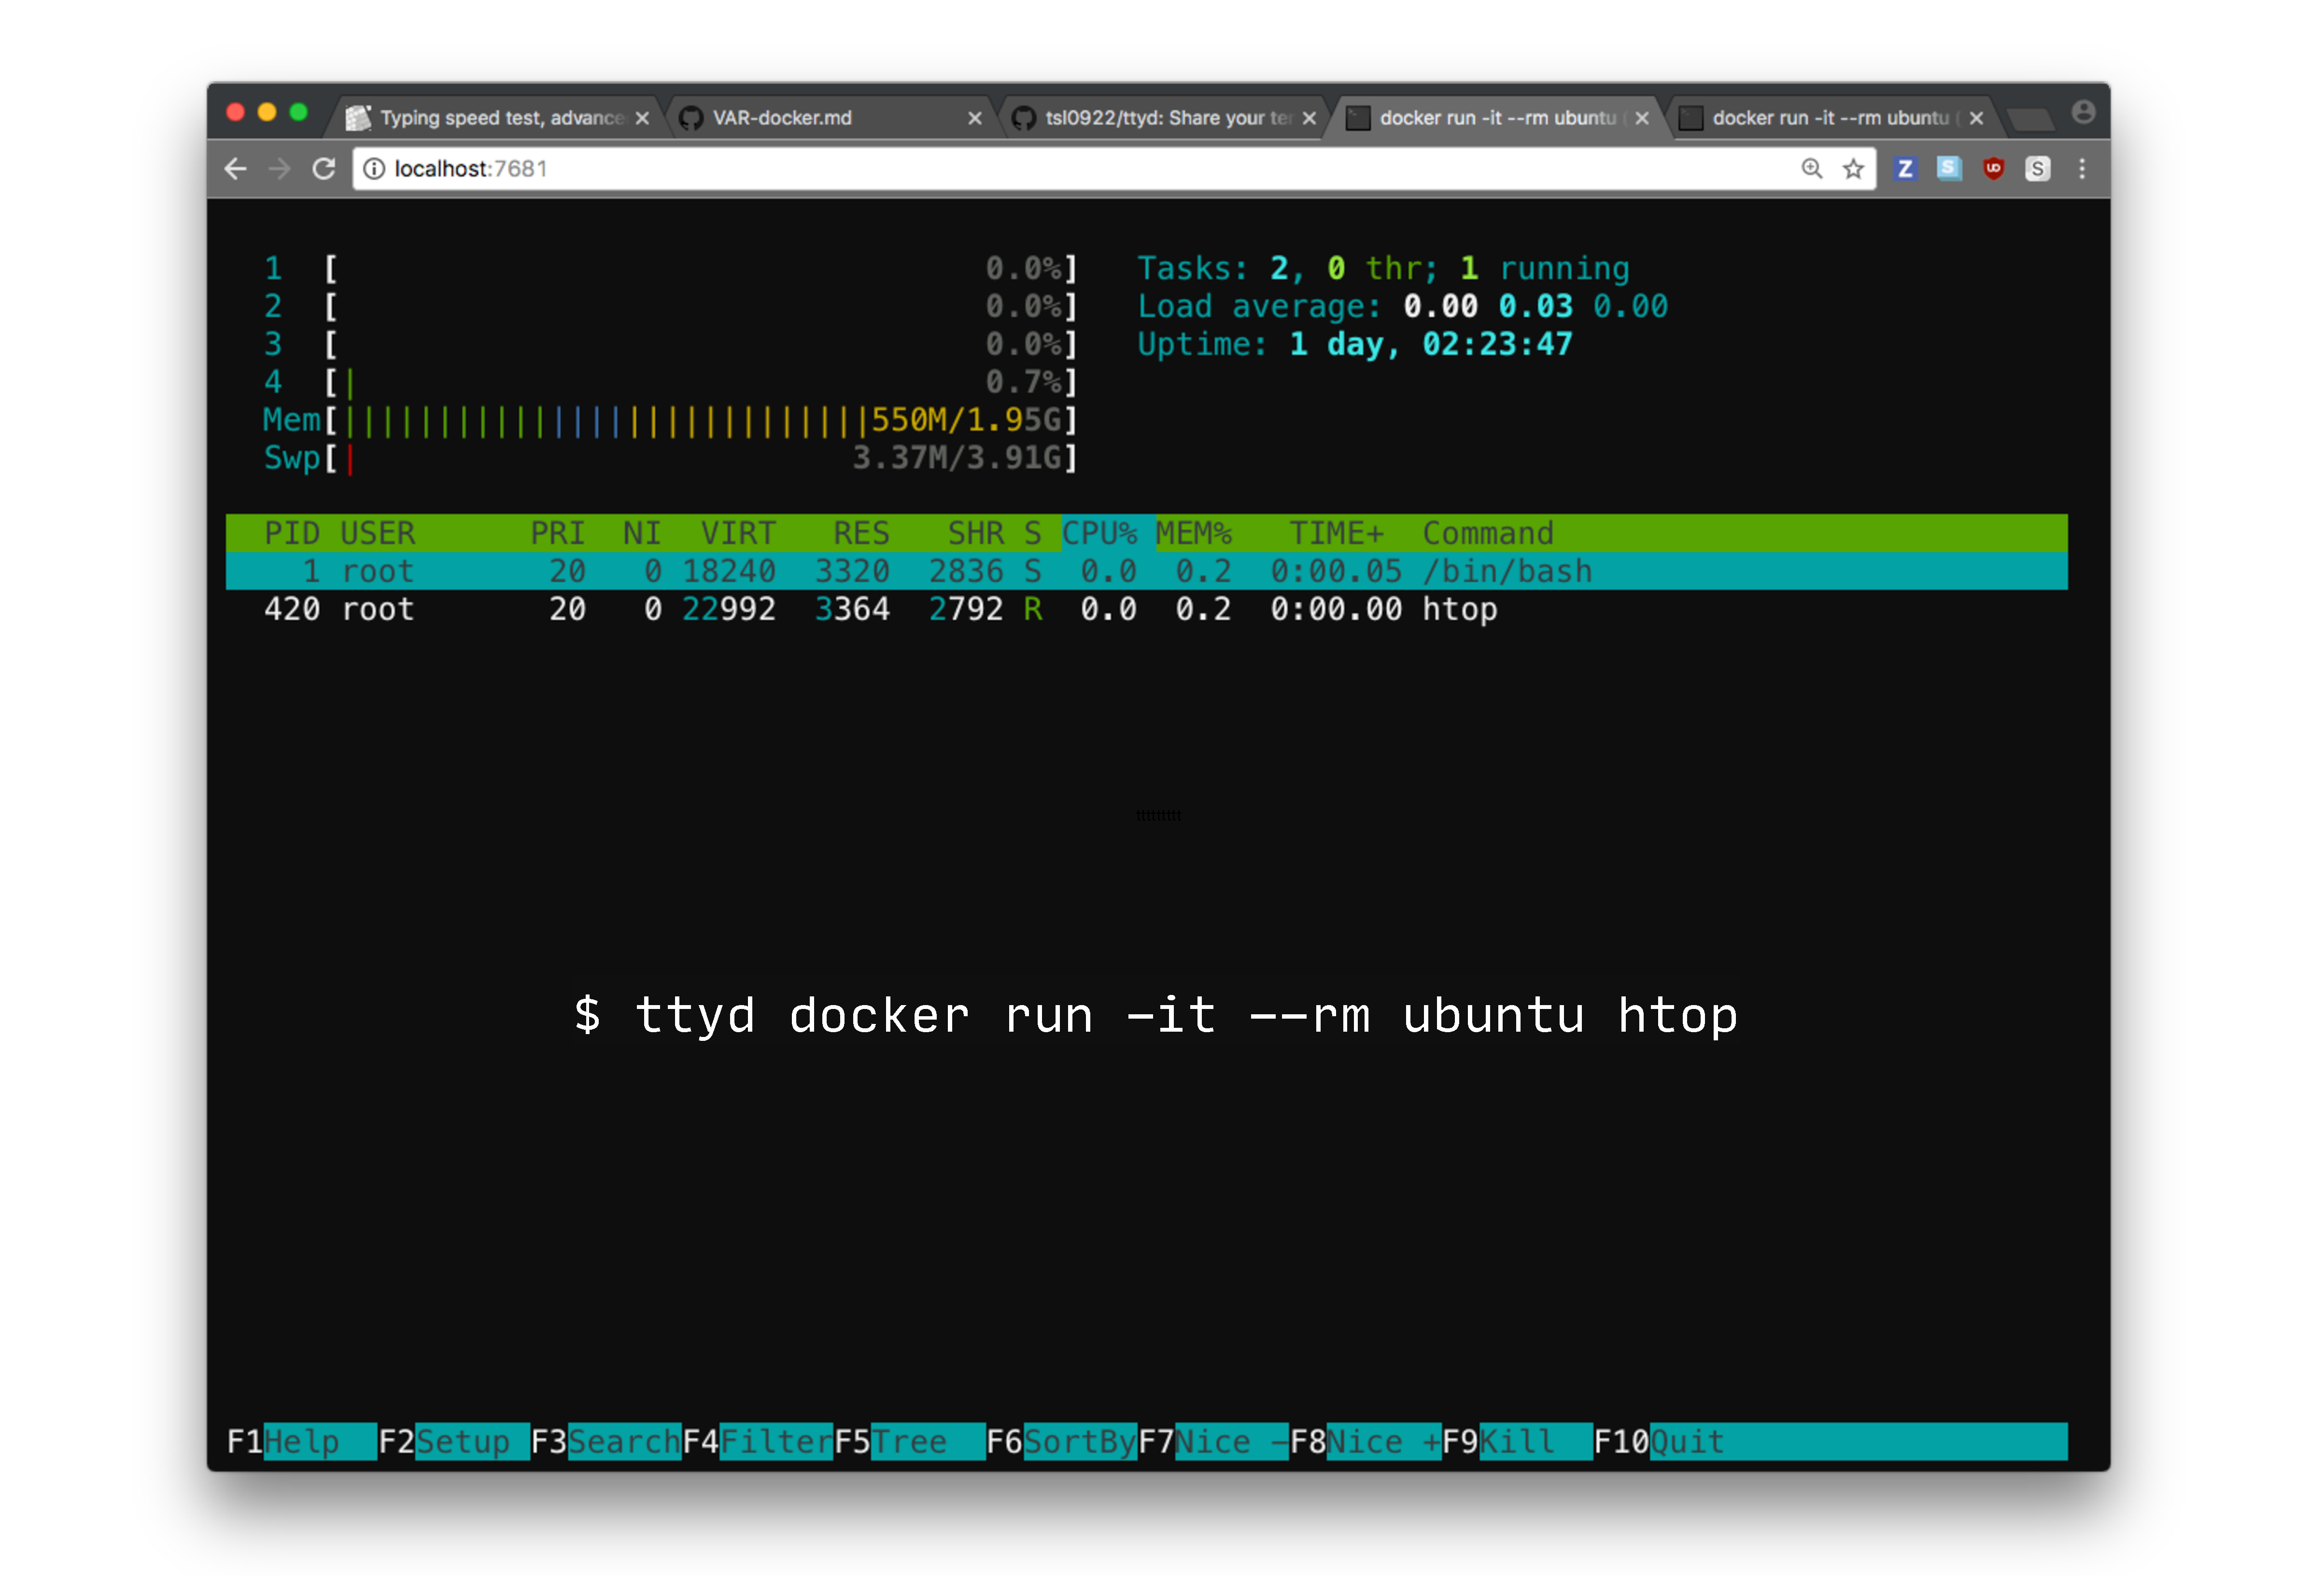
\includegraphics[width=\textwidth]{ttyd.pdf}
\end{frame}

\section{„VAR-Tool“}
\begin{frame}{}
  \AddToShipoutPictureFG*{%
    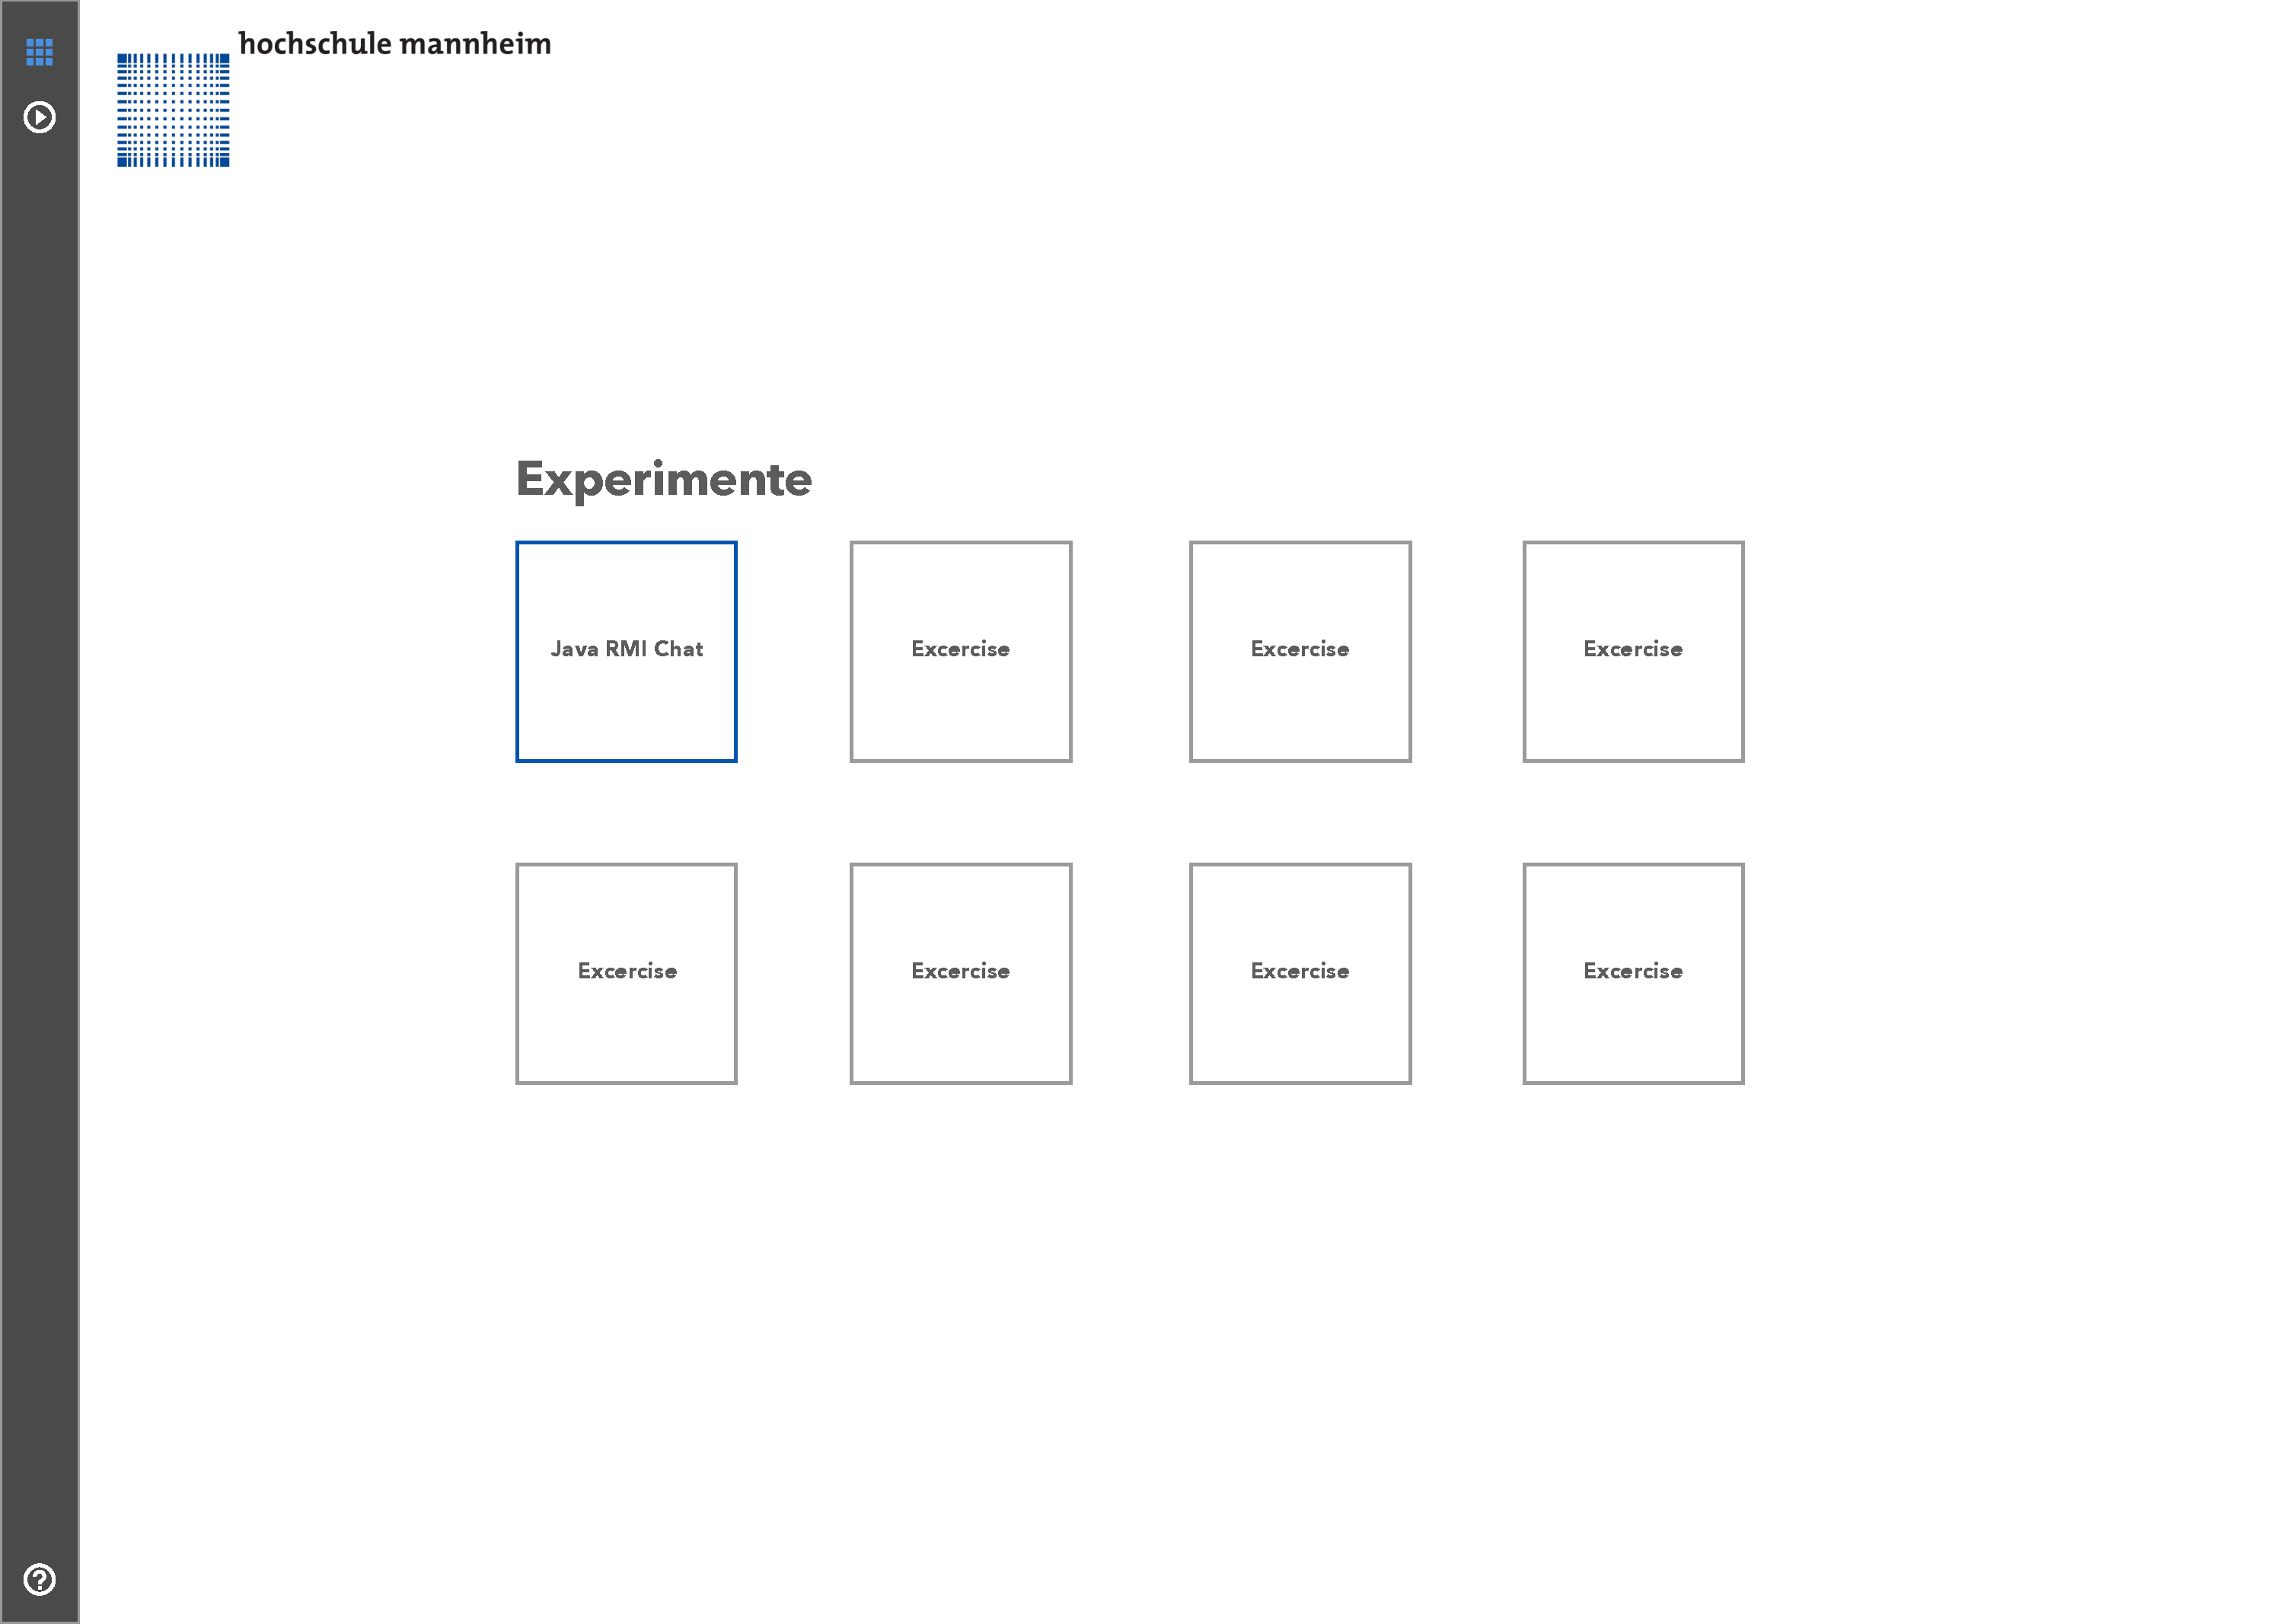
\includegraphics[width=\paperwidth,height=\paperheight,page=1]{ui-mockup.pdf}
  }
\end{frame}
\begin{frame}{}
  \AddToShipoutPictureFG*{%
    \includegraphics[width=\paperwidth,height=\paperheight,page=2]{ui-mockup.pdf}
  }
\end{frame}
\begin{frame}{Network}
  \AddToShipoutPictureFG*{%
    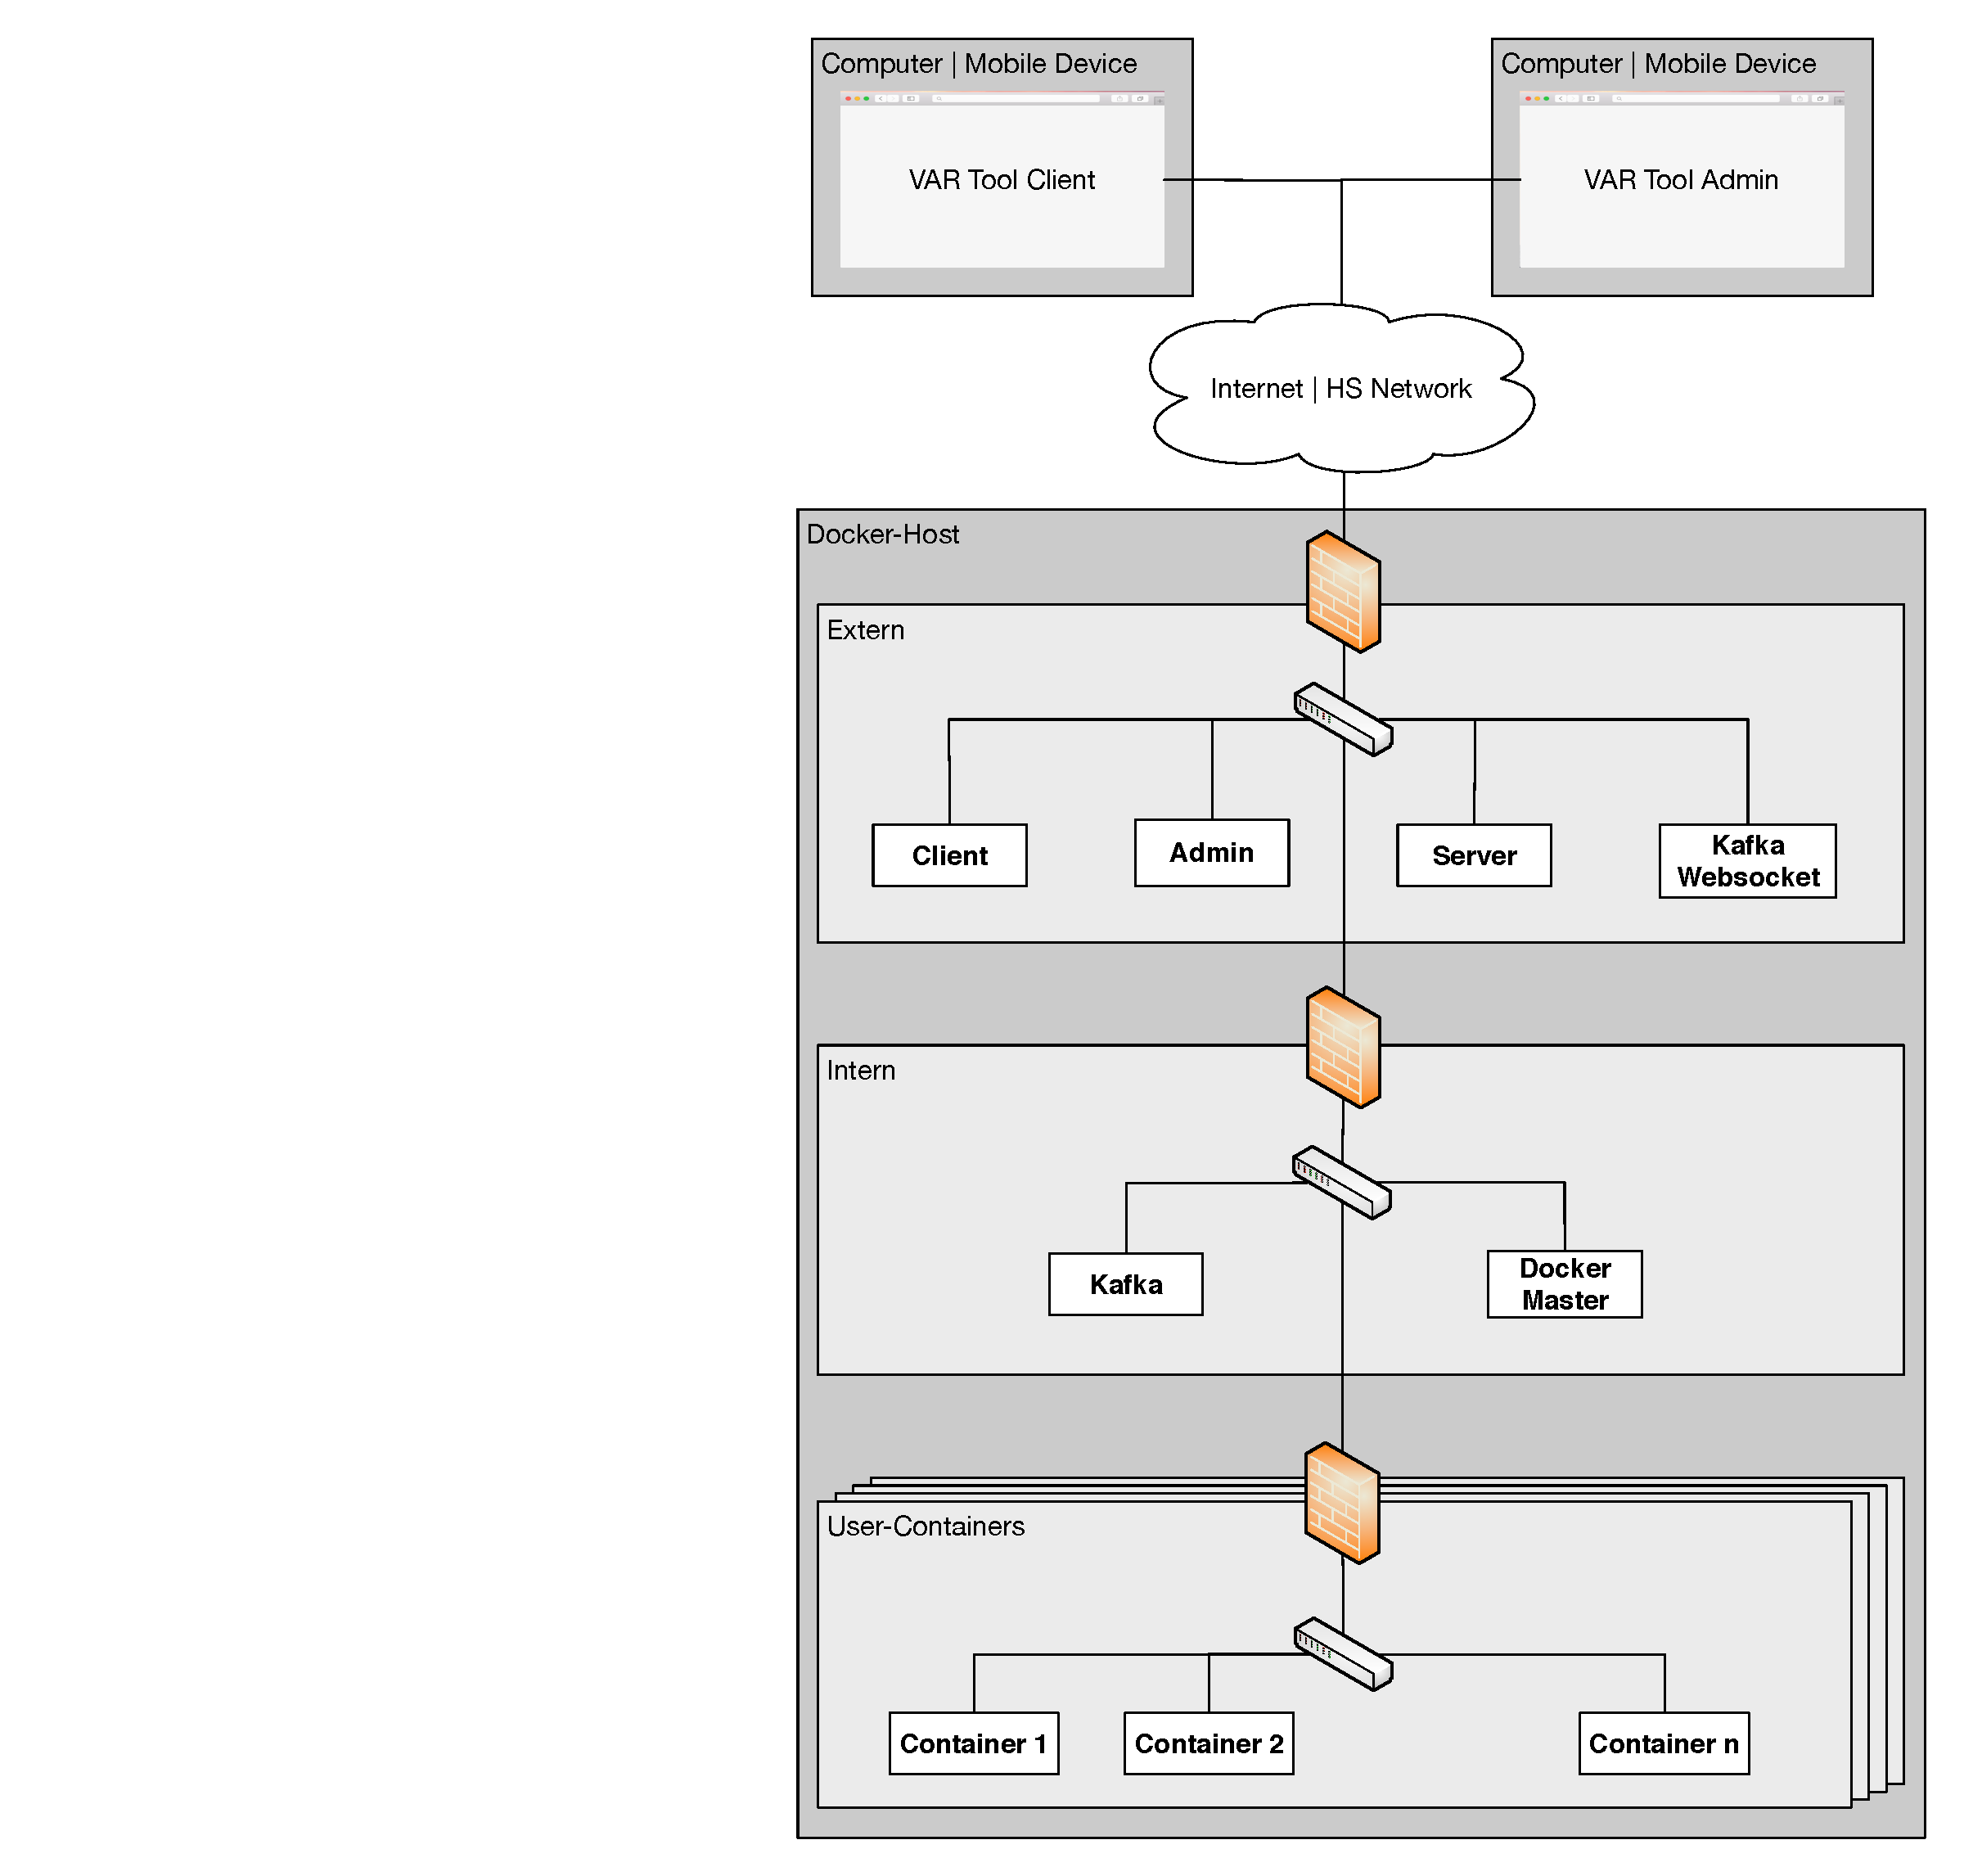
\includegraphics[height=\textheight]{network.pdf}
  }
\end{frame}
\begin{frame}{Sequence}
  \AddToShipoutPictureFG*{%
    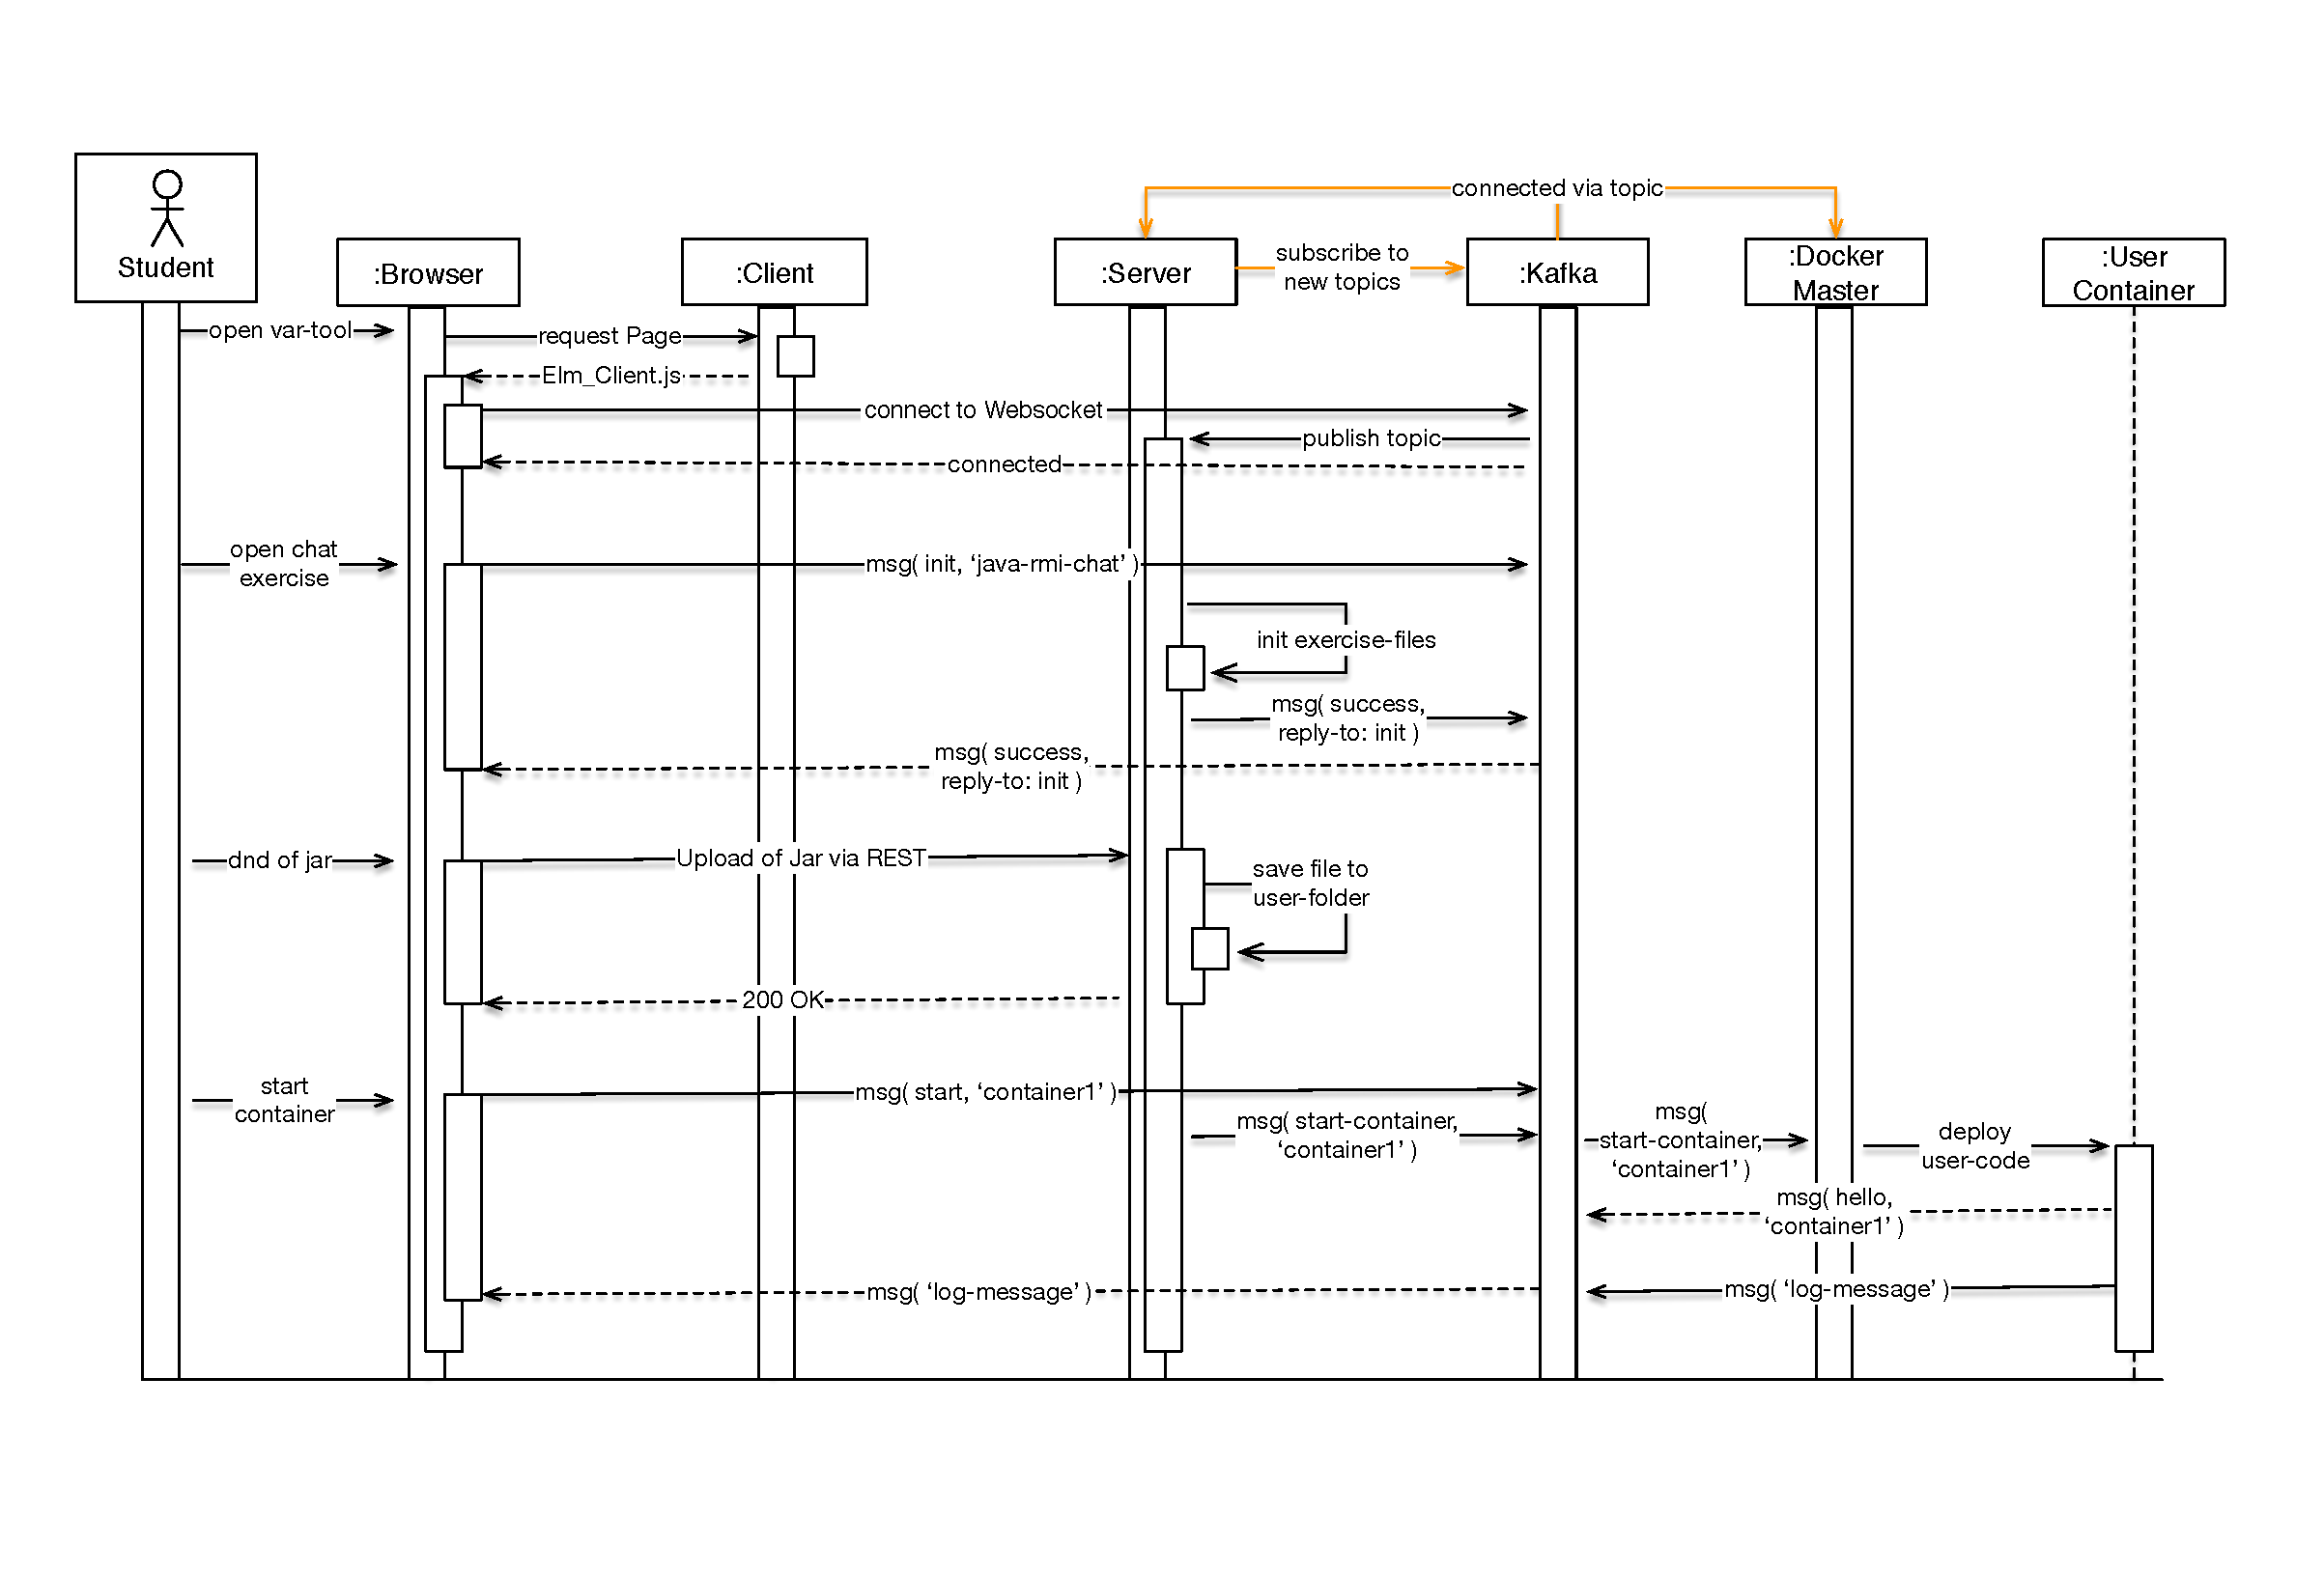
\includegraphics[width=\paperwidth,height=\textheight]{sequence.pdf}
  }
\end{frame}
\begin{frame}{Deployment}
  \AddToShipoutPictureFG*{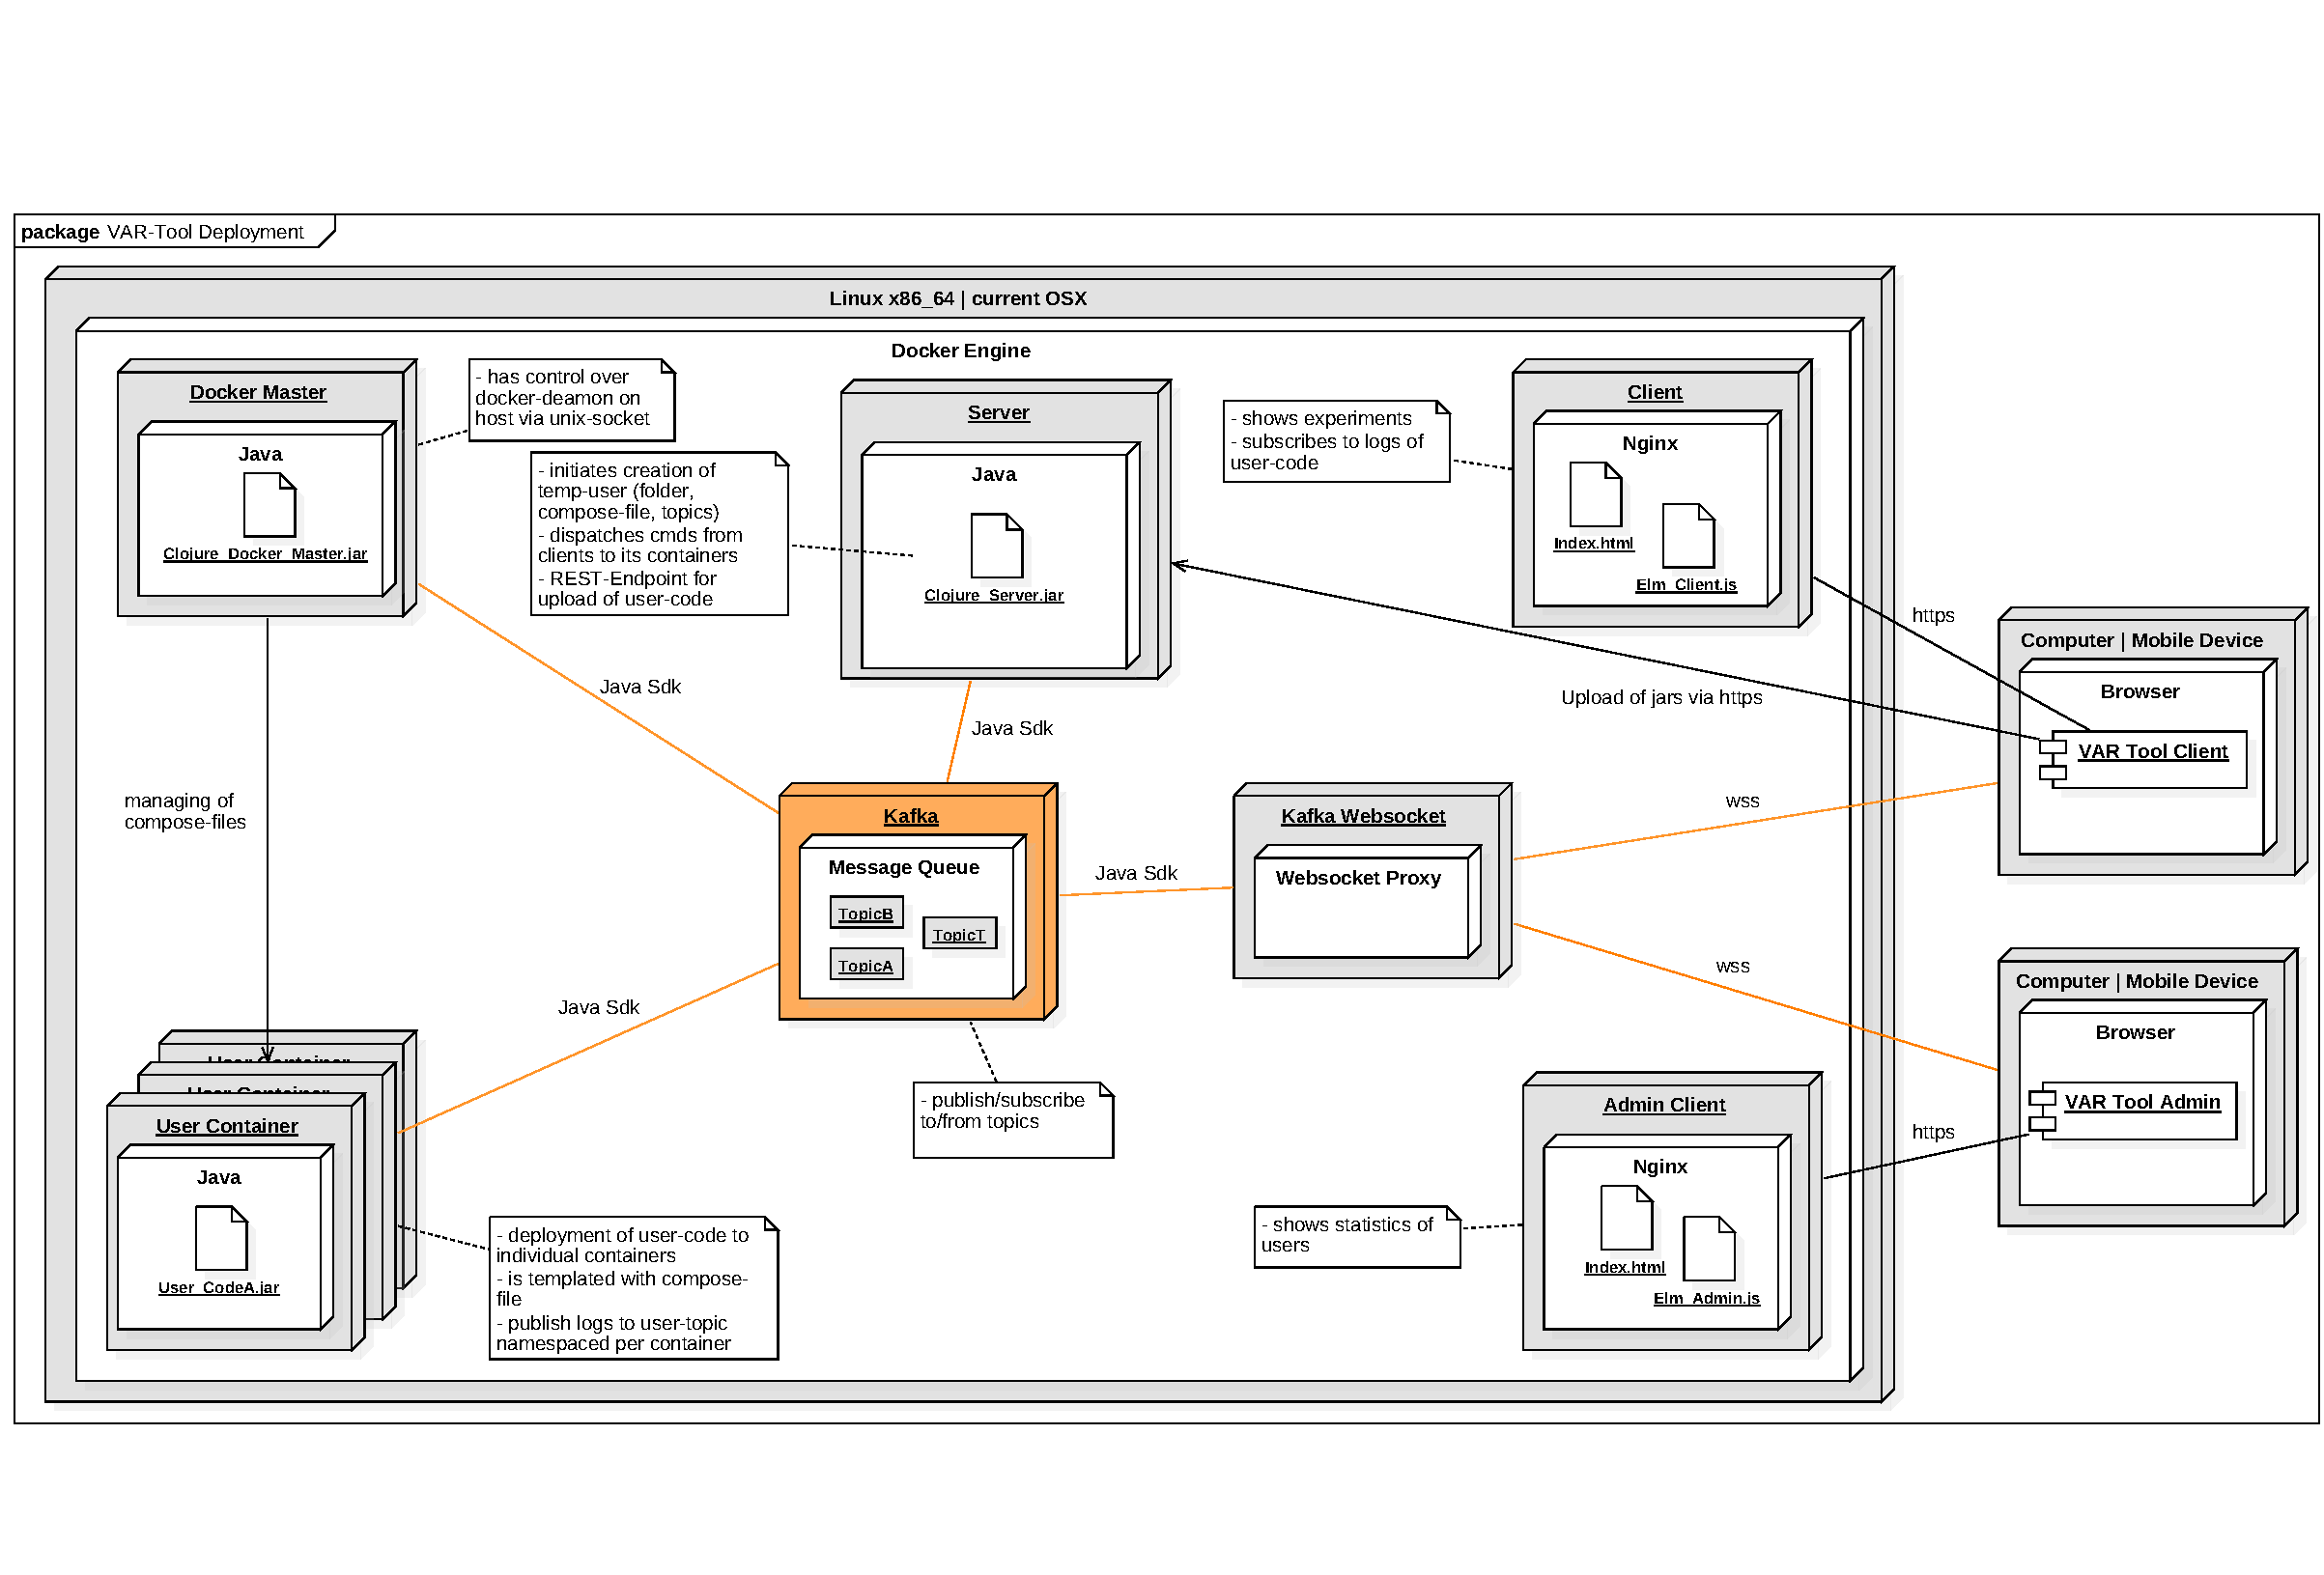
\includegraphics[width=\paperwidth,height=\textheight]{deployment.pdf}}
\end{frame}
\begin{frame}{Compose-File}
  \AddToShipoutPictureFG*{%
    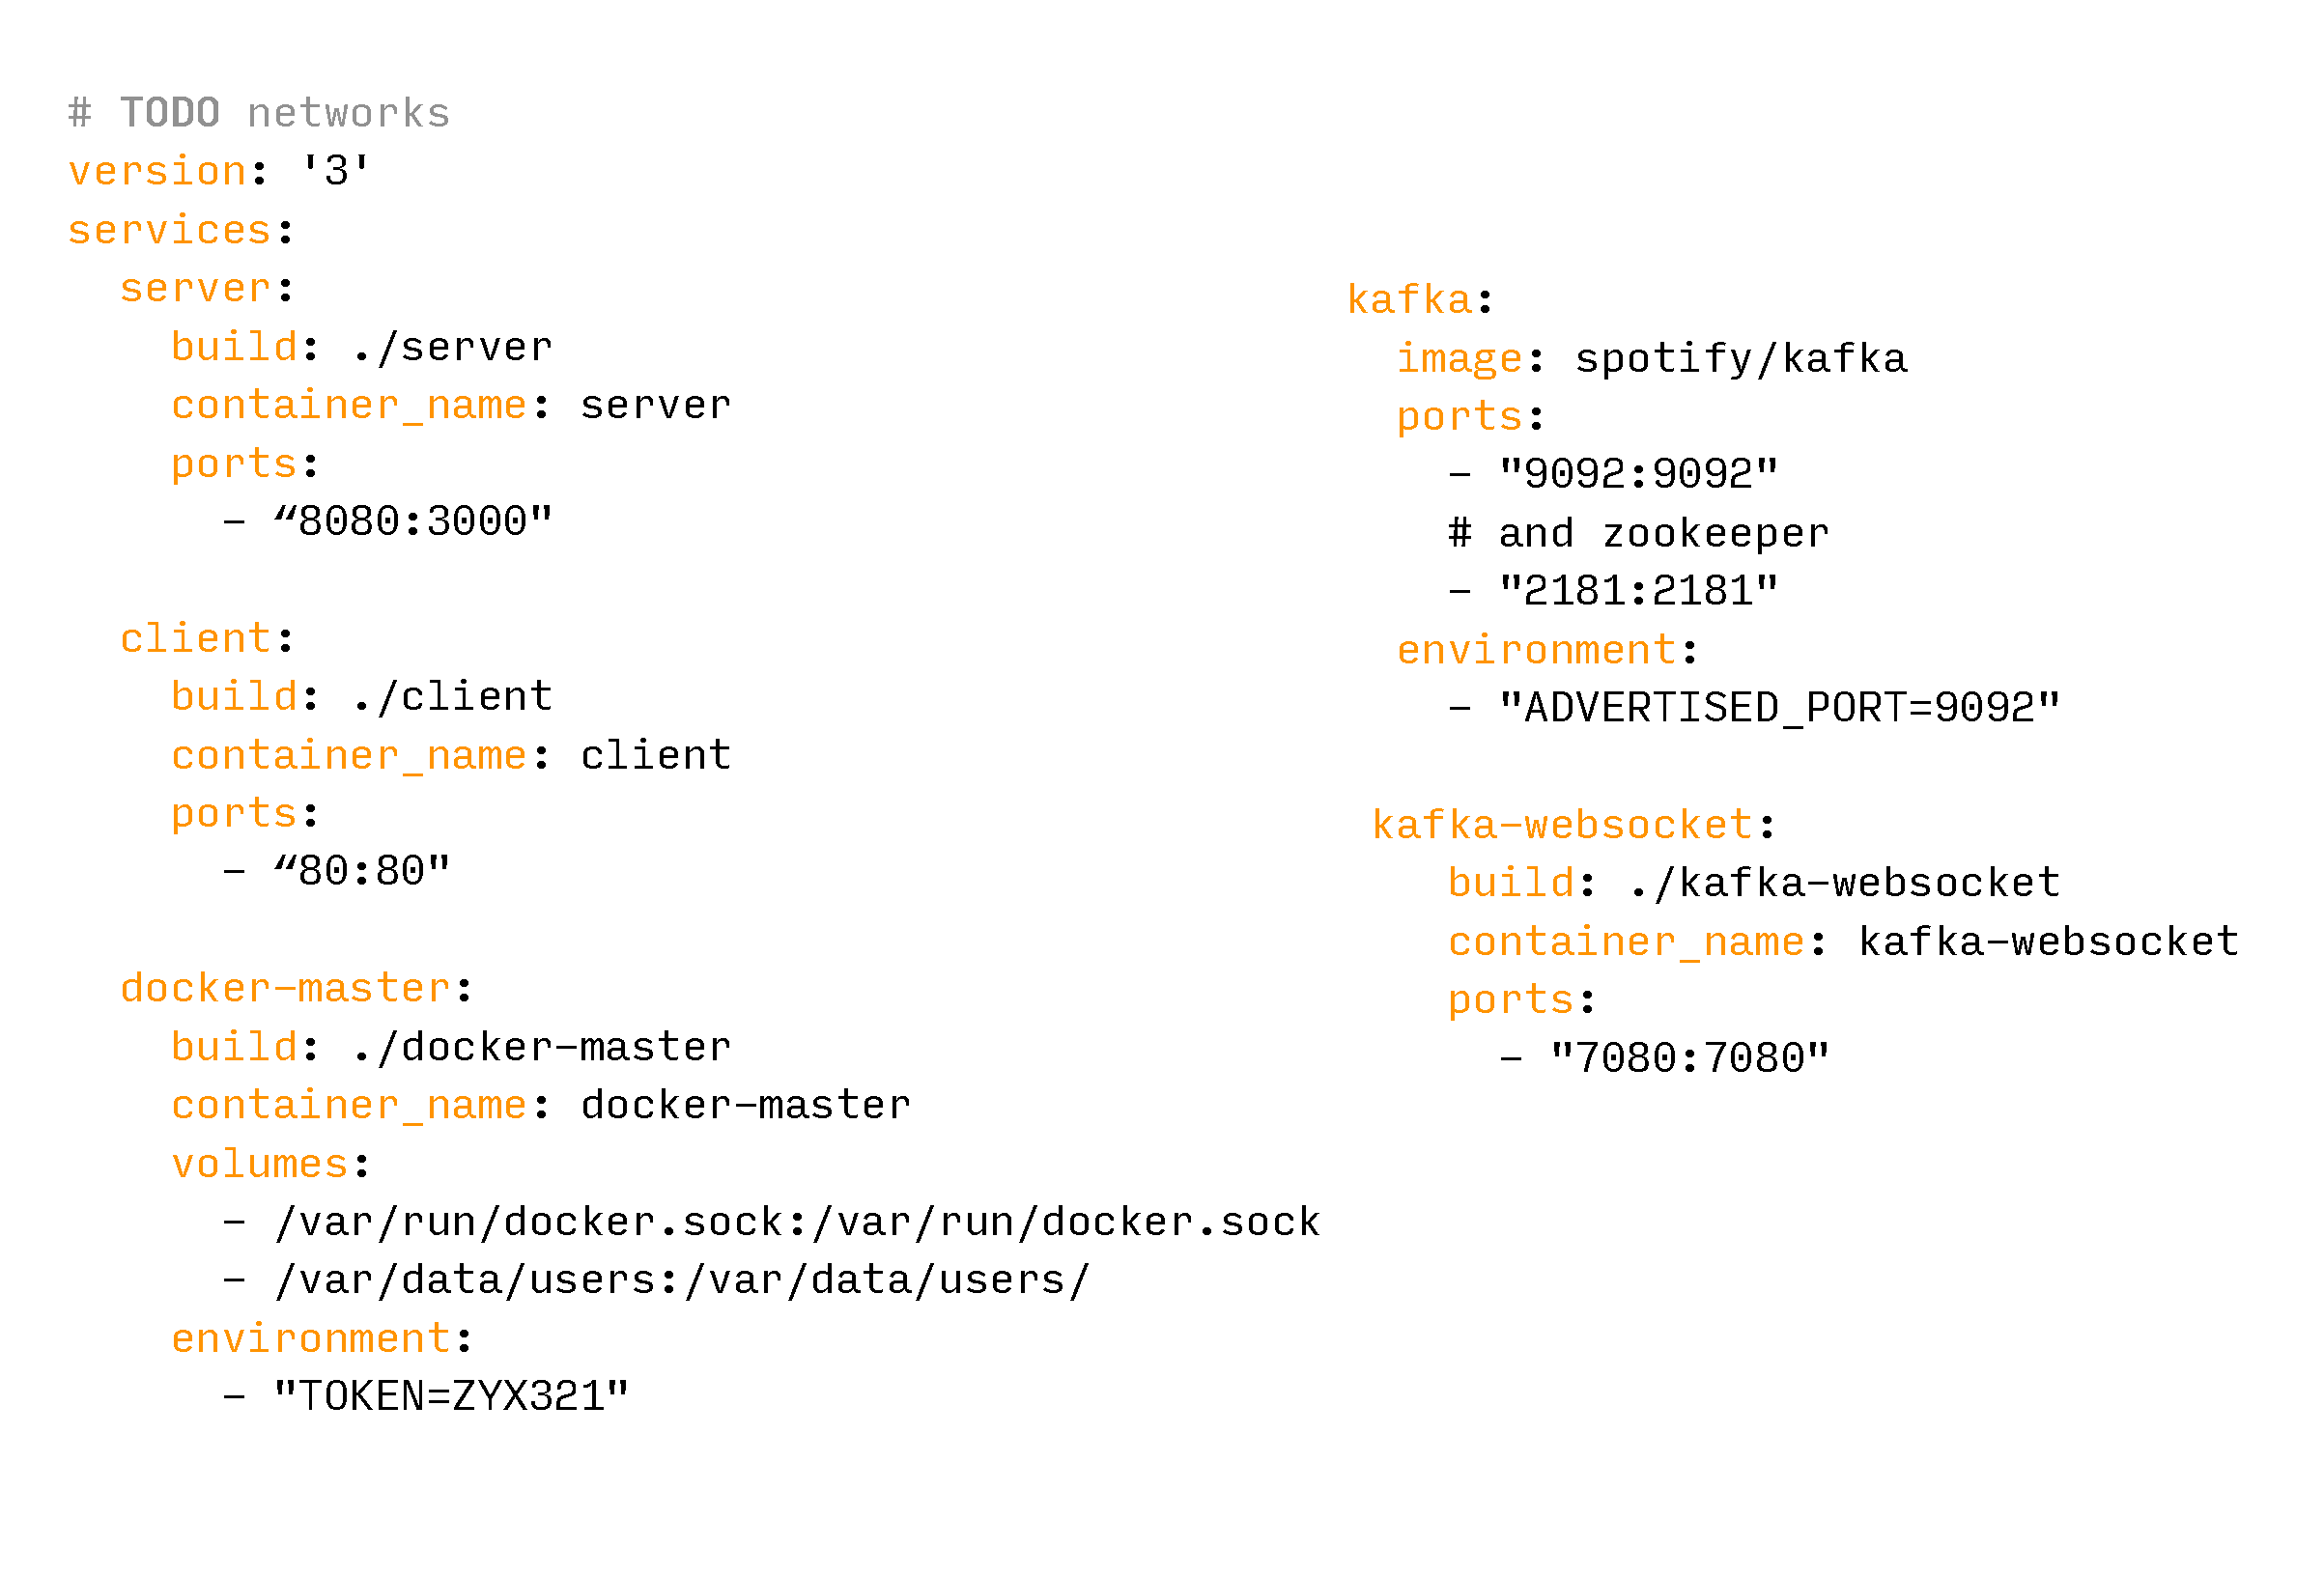
\includegraphics[width=\paperwidth,height=\textheight]{compose.pdf}
  }
\end{frame}

\section{Ausblick}
\begin{frame}{Ausblick \& Fazit}
  \begin{itemize}
    \item EFP: VAR-Tool, Bewertung \& Feedback
    \item Thesis
    \item Veröffentlichung?
  \end{itemize}
  \begin{itemize}
    \item Sehr spannend
    \item Viel Raum für weitere (studentische) Arbeiten
    \item Erstrebenswerte Aufgabe der Fakultät
  \end{itemize}
\end{frame}

\begin{frame}[noframenumbering,plain]{Fin}
  Danke für die Aufmerksamkeit. -- Fragen?
\end{frame}
\end{document}
